% -*- root: ../Crypto.tex -*-
\section{Hoja 1}
\begin{problem}[1]
	Un general espartano recibe el siguiente mensaje de un amigo de Cantoblanco:


	SONFAUHPINPEOCTOHRIANEQLSGCUTUOHEEEQOENRUBSETEIDRELEIT

	¿Qué dice el mensaje?

	\solution
	\doneby{Jorge}

	Si consiguiéramos una escítala cuyo diámetro hiciera que entraran 5 letras por fila conseguiríamos el mensaje:

	SUPONGOQUELOHEHECHOBIENPORQUEESDIFICILTENERTANTASUERTE

\end{problem}

\begin{problem}[2]
	Recibes el mensaje VEILRÑW, cifrado usando una clave de Cesar en el alfabeto castellano de 27 letras (con Ñ y W). Lee el mensaje, da las transformaciones para cifrar y descifrar, y cifra el mensaje GRACIAS utilizando la clave correspondiente.

	\solution
	\doneby{Jorge}

	Usando la transformación:
	\[\appl{f_{17}}{ℤ/27}{ℤ/27}\]
	\[f_{17}(x) = x + 17\]

	Se consigue $f_{17}(\{V,E,I,L,R,Ñ,W\}) = \{M,U,Y,B,I,E,N\}$.

	De modo que para cifrar nos basta:
	\[f_{17}^{-1}(x) = f_{-17}(x) = f_{10}(x)\]
	\[f_{10}(\{G,R,A,C,I,A,S\}) = \{P,B,K,M,R,K,C\}\]
\end{problem}

\begin{problem}[3]
	Utilizando el análisis de frecuencias, descifra el siguiente mensaje, del que sabes que está escrito en inglés (26 letras, con W pero sin Ñ) y que ha sido cifrado con una clave de Cesar:
	PXPXKXENVDRUXVTNLXHYMXGMAXYKXJNXGVRFXMAHWGXXWLEHGZXKVBIAXKMXQM

	\solution
	\doneby{Jorge}

	Al hacer el análisis de frecuencias se obtiene:

	\begin{center}
		\begin{tabular}{ l l }
			P & 0.03225806451612903 \\
			X & 0.24193548387096775 \\
			K & 0.06451612903225806 \\
			E & 0.03225806451612903 \\
			N & 0.04838709677419355 \\
			V & 0.06451612903225806 \\
			D & 0.016129032258064516 \\
			R & 0.03225806451612903 \\
			U & 0.016129032258064516 \\
			T & 0.016129032258064516 \\
			L & 0.03225806451612903 \\
			H & 0.04838709677419355 \\
			Y & 0.03225806451612903 \\
			M & 0.08064516129032258 \\
			G & 0.06451612903225806 \\
			A & 0.04838709677419355 \\
			J & 0.016129032258064516 \\
			F & 0.016129032258064516 \\
			W & 0.03225806451612903 \\
			Z & 0.016129032258064516 \\
			B & 0.016129032258064516 \\
			I & 0.016129032258064516 \\
			Q & 0.016129032258064516
		\end{tabular}
	\end{center}

	Se puede ver que la más frecuente entre todas es la letra X. Si tomamos como letra más usada del ingés la E (en vez de la T) se obtiene el mensaje:

	WEWERELUCKYBECAUSEOFTENTHEFREQUENCYMETHODNEEDSLONGERCIPHERTEXT

	Gracias a la transformación $f_{7}(x) = x + 7$.
\end{problem}

\begin{problem}[4]
	La distribución de frecuencias (en porcentaje) en castellano de las 26 letras (es decir, sin W) es aproximadamente la siguiente.

	\begin{tabular}{c c c c c c c c c c c c c c c c c c c c c c c c c c c}
		A & B & C & D & E & F & G & H & I & J & K & L & M \\
		12,6 & 1,0 & 5,1 & 5,7 & 13,7 & 0,9 & 0,8 & 0,5 & 7,0 & 0,2 & 0,0 & 4,6 & 3,2 \\
		N & Ñ & O & P & Q & R & S & T & U & V & X & Y & Z \\
		7,0 & 0,1 & 8,8 & 2,9 & 1,1 & 6,6 & 7,2 & 5,1 & 3,9 & 0,8 & 0,1 & 0,6 & 0,3
	\end{tabular}

	Recibes un mensaje escrito en castellano (con ese alfabeto) que ha sido cifrado con el criptosistema de Cesar. Las dos letras más frecuentes en el texto cifrado son, por ese orden, la J y la N. Deduce razonadamente cual puede haber sido la clave utilizada para cifrar.

	\solution
	\doneby{Jorge}

	Lo lógico sería que las letras más frecuentes en el alfabeto se correspondieran con las más correspondientes en el mensaje, de modo que lo primero que a uno se le viene a la cabeza es corresponder la J (la más frecuente en el mensaje) con la E (la más frecuente en el alfabeto). Esto viene a ser la transformación $f_{-5}=f_{21}$, la cual manda la N (la segunda más frecuente en el mensaje) a la I (que no es la segunda más frecuente en el español).

	De modo que igual la segunda más frecuente en el mensaje es la que se corresponde con la más frecuente en el alfabeto ($f_{-9}=f_{17}$). Con esta transformación se consigue:
	\[f_{17}(J)=A\]
	\[f_{17}(N)=E\]
	Lo cual es más coherente, ya que hace una correspondencia entre las 2 letras más frecuentes del alfabeto (la E y la A) con las 2 más frecuentes del mensaje.
\end{problem}

\begin{problem}[5]
	Interceptamos un mensaje en el que dos profesores hablan de las asignaturas del plan de estudios de Matemáticas. El mensaje es el siguiente:

	DONQONHOSDGXQKCHDKSNSJSDOQOBDCUQ

	Sabemos que el mensaje ha sido cifrado utilizando una sustitución simple en el alfabeto castellano de 27 letras (con Ñ y W), y sospechamos que en el mensaje original aparecía la palabra CALCULO. Lee el mensaje.

	\solution
	\doneby{Jorge}

	Haciendo el análisis de frecuencias del mensaje interceptado se obtiene:

	\begin{center}
		\begin{tabular}{l l}
			D & 0.15625 \\
			O & 0.15625 \\
			N & 0.09375 \\
			Q & 0.125 \\
			H & 0.0625 \\
			S & 0.125 \\
			G & 0.03125 \\
			X & 0.03125 \\
			K & 0.0625 \\
			C & 0.0625 \\
			J & 0.03125 \\
			B & 0.03125 \\
			U & 0.03125
		\end{tabular}
	\end{center}

	Dentro del mensaje interceptado CALCULO se corresponde con NQONHOS, para darse cuenta basta con fijarse que hayan dos pares de letras iguales al igual que pasa en CALCULO. Con dicha correspondencia de letras tenemos (mostramos el mensaje cortado en 2, donde la fila de debajo de cada trozo se corresponde con lo que llevamos descifrado):

	\begin{center}
		\begin{tabular}{c c c c c c c c c c c c c c c c}
			D & O & N & Q & O & N & H & O & S & D & G & X & Q & K & C & H \\
			\_ & L & C & A & L & C & U & L & O & \_ & \_ & \_ & A & \_ & \_ & U
		\end{tabular}
	\end{center}

	\begin{center}
		\begin{tabular}{c c c c c c c c c c c c c c c c}
			D & K & S & N & S & J & S & D & O & Q & O & B & D & C & U & Q \\
			\_ & \_ & O & \_ & O & \_ & O & \_ & L & A & L & \_ & \_ & \_ & \_ & A
		\end{tabular}
	\end{center}

	Puesto que el análisis de frecuencias nos dice que la D es la letra que más aparece, probaremos a corresponderla con la letra E:

	\begin{center}
		\begin{tabular}{c c c c c c c c c c c c c c c c}
			D & O & N & Q & O & N & H & O & S & D & G & X & Q & K & C & H \\
			E & L & C & A & L & C & U & L & O & E & \_ & \_ & A & \_ & \_ & U
		\end{tabular}
	\end{center}

	\begin{center}
		\begin{tabular}{c c c c c c c c c c c c c c c c}
			D & K & S & N & S & J & S & D & O & Q & O & B & D & C & U & Q \\
			E & \_ & O & \_ & O & \_ & O & E & L & A & L & \_ & E & \_ & \_ & A
		\end{tabular}
	\end{center}

	Fijándonos en que la K y la C son las siguientes letras con mayor frecuencia, y que de entre las no utilizadas del alfabeto, la S y N son las siguientes que tienen más frecuencia en español. Probando se llega a que la K va a la N, y la C a la B.

	\begin{center}
		\begin{tabular}{c c c c c c c c c c c c c c c c}
			D & O & N & Q & O & N & H & O & S & D & G & X & Q & K & C & H \\
			E & L & C & A & L & C & U & L & O & E & \_ & \_ & A & N & B & U
		\end{tabular}
	\end{center}

	\begin{center}
		\begin{tabular}{c c c c c c c c c c c c c c c c}
			D & K & S & N & S & J & S & D & O & Q & O & B & D & C & U & Q \\
			E & N & O & \_ & O & \_ & O & E & L & A & L & \_ & E & B & \_ & A
		\end{tabular}
	\end{center}

	Llegados a este punto, somos capaces de adivinar que lo que pone el mensaje es:

	EL CALCULO ES TAN BUENO COMO EL ALGEBRA
\end{problem}


\begin{problem}[6]
	Interceptamos cuatro mensajes cifrados. Sabemos que tanto los mensajes en claro como los mensajes cifrados han sido escritos utilizando el alfabeto inglés de 26 letras. Las frecuencias con que cada letra aparece en cada mensaje son las siguientes:

	\begin{center}
		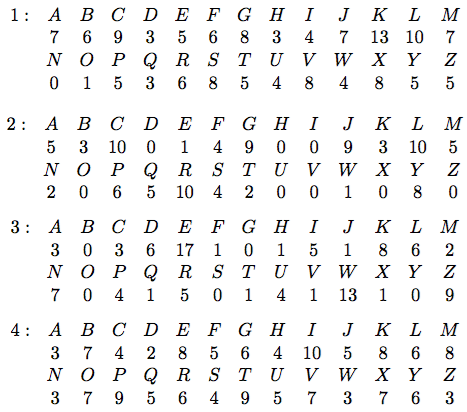
\includegraphics[width=0.5\textwidth]{img/freqsEj1_6}
	\end{center}

	¿Cuáles de los mensajes es razonable pensar que han sido cifrados utilizando sustituciones simples sobre letras?

	\solution
	\doneby{Pedro}

	Lo único que podemos hacer es fijarnos en las frecuencias de las diferentes letras y ver en qué mensajes las letras tienen unas frecuencias similares a las del inglés.

	Basándonos en la tabla de frecuencias de moodle podemos agrupar las letras del alfabeto inglés según la frecuencia con que se usan (en inglés y en cada uno de los mensajes interceptados).

	Si la columna de un mensaje se asemeja a la segunda columna, ese mensaje tendrá alta probabilidad de haber sido cifrado empleando una sustitución simple sobre letras.

	\begin{center}
	\begin{tabular}{| c | c || c | c | c | c |}
	\hline
	\textbf{Porcentaje} & \textbf{Nº Ingles} & \textbf{Nº M1} & \textbf{Nº M2} & \textbf{Nº M3} & \textbf{Nº M4} \\
	\hline
	0-2 & 10 & 2 & 9 & 12 & 0\\
	\hline
	2-4 & 6 & 3 & 4 & 3 & 5 \\
	\hline
	4-6 & 1 & 8 & 5 & 3 & 7 \\
	\hline
	6-8 & 7 & 6 & 1 & 3 & 8 \\
	\hline
	8-10 & 1 & 5 & 3 & 2 & 5 \\
	\hline
	>10 & 1 & 2 & 3 & 2 & 1 \\
	\hline
	\end{tabular}
	\end{center}

	Antes de nada hay que comentar que no sabemos qué longitud tenía cada mensaje por lo que tampoco sabemos cómo de válidas son las frecuencias calculadas. Por ello se ha tomado la decisión de agrupar las frecuencias por valores.

	Si sabemos que cada mensaje era un ``Los Pilares de la Tierra'' en inglés y cifrado, tendremos unas estimaciones de la frecuencia de cada letra muy muy buenas, por lo que podríamos agrupar las frecuencias por unidades.

	El primer y el último mensajes tienen muy pocas letras con baja frecuencia y demasiadas con frecuencia 8-10 por lo que parece razonable descartar la posibilidad de que hayan sido escritos en inglés.

	Entre el segundo y el tercero, el que más posibilidades tiene de haber sido escrito originalmente en inglés es el tercero, pues el segundo tiene muy pocas letras con frecuencia 6-8 y quizás demasiadas con frecuencias altas.

	Para el espía experto otra posibilidad sería estudiar la media y la varianza de la distribución de frecuencias en cada mensaje y apoyarse también en eso a la hora de tomar la decisión.
\end{problem}


\begin{problem}[7]
	En un alfabeto de 28 letras, las 27 del castellano y el espacio=27, utiliza la clave afíın sobre letras $f(m) = 13m + 9$ para cifrar el mensaje ``MUY BIEN''.

	\solution

	\doneby{Jorge}

	Utilizamos el $\_$ para representar el espacio y que este se vea claro.
	\[f(``MUY\_BIEN'')=``SXTRPW\_E''\]
\end{problem}


\begin{problem}[8]
	Sabemos que el enemigo está utilizando transformaciones afines sobre letras para cifrar mensajes escritos en inglés con el siguiente alfabeto de 37 letras: los números 0,...,9 que se codifican como ellos mismos; las letras A,…,Z (con W, sin Ñ), que corresponden a 10,…,35; y el espacio en blanco=36. Interceptamos el siguiente mensaje cifrado

	OH7F86BB46R3627O266BB9 (Atención, no hay ceros, sólo os)

	Sabiendo que el mensaje original acaba con la firma 007 (cero, cero, siete), ¿qué dice el mensaje?

	\solution
	\doneby{Jorge}

	La transformación afín será de la forma:
	\[ f_{a,b}(x) = ax+b \]

	Luego planteando un sistema de ecuaciones obtenemos a y b, sabemos que B=11:
	\[ f_{a,b}(11) = a·11 + b = 0\]
	\[ f_{a,b}(9)  = a·9  + b = 7 \]

	\[ b = -11a = 26a \]

	Luego
	\[ 9a + 26a = 35a = 7 \implies a = 15  \implies b = 20\]

	Aplicando $f_{a,b}$ al mensaje cifrado se obtiene:
	\begin{center}
		``AGENT 006 IS DEAD  007''
	\end{center}
\end{problem}


\begin{problem}[9]
	Una unidad de texto (en claro) m se dice que es fija para una transformación para cifrar si $f(m) = m$. Supongamos que estamos usando transformaciones afines sobre letras en un alfabeto de N letras, $f(m) = a · m + b$ con $a ≠ 1$.

	\begin{enumerate}
		\item Demostrar que si N es primo hay exactamente una letra fija.
		\item Demostrar que para N arbitrario cualquier transformación lineal (es decir, con b = 0) tiene al menos una letra fija, y que si N es par cualquier transformación lineal tiene al menos dos letras fijas.
		\item Dar un ejemplo de una transformación afín (para algún N) sin letras fijas.
	\end{enumerate}

	\solution
	\doneby{Jorge}
	\begin{enumerate}
		\item $m = a · m + b  \implies (a-1)·m + b = 0 \implies m = -(a-1)^{-1} · b$. En caso de que $N$ sea primo sabemos que existe $(a-1)^{-1}$, ya que en ese caso $U(ℤ/N)=ℤ/N$ y por tanto $(a-1) ∈ U(ℤ/N)$. Así que $m$ es único al quedar determinado por el producto de $(a-1)^{-1}$ y $b$.

		\item En caso de que $f(m) = a·m$ sabemos que siempre tendremos la letra fija asociada al 0 (ya que $f(0)=0$) independientemente de qué $N$ tengamos.

		Si $f(m) = a·m$ con $N$ par ($N=2M$), se cumple, además, que $f(M)=M$, ya que

		\[f(M)=M \iff aM = M \iff (a-1)M = 0 \iff 2M | (a-1)M \]

		Y puesto que $a$ debe ser unidad en $\ent_{2M}$, debe ser coprimo con $2M$ y, por tanto, impar. Por tanto, es claro que $(a-1)$ será par y, efectivamente $(a-1)M = k \cdot 2M$

		\item Para $N=2$ la transformación $f(x) = x + 1$ no deja letras fijas.
	\end{enumerate}
\end{problem}

\begin{problem}[10]
	Sea $A$ un anillo conmutativo con 1. Diremos que $a∈A$ es un divisor de 0 si existe $b∈A$, $b≠0$ y tal que $ab = 0$ (con esta definición, que no es la normal, 0 es un divisor de 0, pero no importa, simplifica los enunciados). Diremos que $a ∈ A$ es una unidad si existe $b ∈ A$ tal que $ab = 1$.

	\ppart Demostrar que $\left\{ \text{Unidades de } A \right\} ∩ \left\{ \text{Divisores de 0 en } A \right\} = \emptyset$
	\ppart Dado $a ∈ A$, definimos la aplicación ``multiplicar por $a$'', $\appl{m_a}{A}{A}$ como $m_a(x) = ax$. Caracterizar los divisores de 0 (o quizá los no divisores de 0) y las unidades de $A$ en términos de propiedades de la correspondiente aplicación $m_a$.
	\ppart Utilizar la caracterización anterior para demostrar que si $A$ es un anillo finito se tiene:

		\[\left\{ \text{Unidades de } A \right\} \cup \left\{ \text{Divisidores de 0 en } A \right\} = A\]

		(Esto generaliza lo que sucede en los anillos de congruencias $ℤ/Nℤ$.)
	\ppart Demostrar que la hipótesis de finitud es esencial en el apartado 3.

	\solution
	\doneby{Pedro}

	\spart
	Supongamos que tenemos un elemento $x$ que es unidad y divisor de 0 simultáneamente.

	En ese caso tendríamos que existen dos números $a$ y $b$, ambos distintos de 0, tales que: $ax = 0$ y $bx = 1$

	En esta situación podemos tomar la ecuación $bx=1$ y multiplicar por $a$ a ambos lados, con lo que mantenemos la igualdad, obteniendo:
	\[bx = 1 \iff abx = a \iff axb = a \iff 0 \cdot b = a \iff 0 = a\]

	Con lo que llegamos a una contradicción, pues dijimos que $a \neq 0$

	\spart

	Si tenemos que $a$ es un divisor de 0, habrá algún valor (distinto de 0) que nos llevará a 0, con lo que la función $f_a$ no será inyectiva.

	A raíz de esto podemos ver que si $a$ no es un divisor de 0, la función $m_a(x)=ax$ será inyectiva. Para comprobarlo basta con ver que:
	\[\forall x\neq y, \ ax=ay \implies a(x-y)=0 \implies a \text{ divisor de 0 ya que } x-y \neq 0\]
	lo que nos lleva a una contradicción.

	Por otro lado, si $a$ es una unidad, la función será sobreyectiva pues tendremos:
	\[\forall y \ ax = y \implies x = ya^{-1} \implies \exists x \tq m_a(x)=y\]

	Además, de esta misma fórmula podemos deducir que si no es unidad, no será sobreyectiva la función (no podremos llegar al 1, por ejemplo)

	\spart

	Si tenemos un elemento $a \in A$ que no es unidad ni divisor de 0 en $A$, tendremos que la función asociada $m_a$ será inyectiva pero no sobreyectiva.

	Si una función entre dos conjuntos finitos es inyectiva pero no sobreyectiva, esto implica que el conjunto de partida es menor que el de llegada. Pero por definición, la función $m_a$ va de un conjunto en si mismo, con lo que es imposible que sea inyectiva y no sobreyectiva.

	Por tanto es imposible que exista un $a$ como el que hemos definido. Es decir, tenemos demostrado que
	\[\left\{ \text{Unidades de } A \right\} \cup \left\{ \text{Divisidores de 0 en } A \right\} \supset A\]

	El otro sentido del contenido es trivial por la propia construcción del conjunto de unidades y de los divisores.

	\spart

	Si $A$ se tratase del anillo $(\ent, +, \cdot )$, dado $a=2$ podemos construir una aplicación $m_a$ que, como se probó en el apartado anterior, sería inyectiva pues 2 no es divisor de 0.

	Sin embargo, al no ser un cuerpo finito no hay problema en que una función vaya de un anillo en si mismo siendo inyectiva pero no sobreyectiva. Por tanto no podríamos deducir ninguna relación de contención.

	\doneby{Edu}

	\spart[a]

	Supongamos x $\in \text{Unidades de } A$ y $\exists y \neq 0 \tq x\cdot y = 0$, ie, x $\in \text{Divisores de 0 en } A$:
	\[ x \cdot y = 0 \implies x^{-1} \cdot x \cdot y = 0 \implies y = 0 \Rightarrow \Leftarrow \]
	{\bf Conclusión:} si x $\in \text{Unidades de } A \implies$ x $\not\in \text{Divisores de 0 en } A$

	Supongamos x $\in \text{Divisores de 0 en } A$, ie, $\exists y \neq 0 \tq x \cdot y = 0$ y supongamos $\exists z \neq 0 \tq x \cdot z = 1$:
	\[ x \cdot z = 1 \implies y \cdot x \cdot z = y \cdot 1 \implies 0 \cdot z = y \implies 0 = y \Rightarrow \Leftarrow \]
	{\bf Conclusión:} si x $\in \text{Divisores de 0 en } A  \implies$ x $\not\in \text{Unidades de } A$
	\newline\qed

	\spart[b]

	Si $m_a$ es inyectiva (y {\bf por ser A finito} entonces es sobreyectiva)

	$\implies \forall x,y \neq 0 \in A$, $m_a(x) = xa = ya = m_a(y) \implies x = y \implies $ a $\in $ unidades de A ya que, al ser {\bf sobreyectiva}, $\exists y \in A \tq a\cdot y = 1$.

	Si $m_a$ no es sobreyectiva, ie, GCD($m\cdot a$, |A|) $> 1$ para algún a, $\exists x,y \in A, x \neq y \tq$ $a \cdot x = a \cdot y \implies a (x - y) = 0 \implies a$ es divisor de 0.

	\spart[c]

	Como observación, diremos que si la afirmación es falsa, por el apartado 1, tiene que existir un $x$ que no pertenece a ninguno de los dos subconjuntos de A, lo cual es imposible por el apartado anterior: si $m_a$ es inyectiva, entonces $a$ es unidad, si $m_a$ no es sobreyectiva, $a$ es divisor de 0.
\newline\qed

	\spart[d]

	Leer la parte negrita del apartado B y convencerse de que no tiene por qué existir el inverso de $a$.

\end{problem}





\section{Control 1 (22-09-2014) Modelo A}
\begin{problem}[1]
Dado $N\geq 2$ y un elemento $a \in \ent_N$, consideramos la aplicación $\appl{m_a}{\ent_N}{\ent_N}$ tal que $m(x)=ax$.

Demostrar que son equivalentes:
\begin{enumerate}
\item $a$ es unidad en $\ent_N$
\item $a$ y $N$ son primos entre si.
\item $m_a$ es inyectiva
\item $m_a$ es sobreyectiva
\end{enumerate}

\solution
\doneby{Pedro}

Para demostrar que los enunciados son equivalentes vamos a demostrar una serie de implicaciones de modo que, al final, desde cualquiera de esas afirmaciones podamos llegar a cuaquier otra.

\begin{itemize}
\item \textbf{$1 \implies 2$}
Si $a$ es una unidad en $\ent_N$ sabemos que existe $c \in \ent_N$ tal que
\[ac = kN + 1\]

Supongamos ahora que $a$ y $N$ no son primos entre si, es decir,
\[\exists b \tq a = b \cdot a' \text{ y } N = b \cdot N'\]

Sustituyendo en la primera fórmula obtenemos
\[ba'c=bkN'+1 \iff b(a'c-kN')=1 \iff b \in U(\ent_N)\]

Pero está claro que $b$ no puede pertenecer a las unidades de $\ent_N$ ya que, siempre que $bc< N$ es claro que $bc \neq 1$ salvo que ambos sean 1 y, además:
\[\forall c \in \ent_N, \tq cb > N \iff cb = bN'α+bβ \text{ siendo } bβ < N\]
con lo que el resto nunca será 1.

\item \textbf{$2 \implies 3$}

Ahora tenemos $a$, $N$ tales que $(a,N)=1$ y queremos ver que la función $m_a$ es inyectiva.

Suponemos que no es inyectiva y que por tanto $\exists x,y \in \ent_N$ tales que $x \neq y$ y:
\[ax=ay \text{ mod } n \iff a(x-y)= 0 \ \text{mod } n \iff a(x-y) = c N\]

Pero, en caso de ser esto cierto, por definición, $a$ sería un divisor de $cN$ y, por tanto, $a$ divide a $c$ ya que estamos considerando $(a,N)=1$.

Si $a$ fuese divisor de $c$, podríamos escribir:
\[a(x-y)=kaN \iff (x-y) = kN\]
pero consideramos que $x$ y $y$ son dos elementos distintos de $\ent_N$ y, por tanto, su diferencia no puede ser múltiplo de $N$. Con lo que llegamos a una contradicción.

Por tanto no pueden existir $x$, $y$ como los descritos con lo que queda claro que la función es inyectiva.

\item \textbf{$3 \implies 4$}
Como estamos moviéndonos en un conjunto finito, si la función es inyectiva debe ser también sobreyectiva.

\item \textbf{$4 \implies 1$}

Si la función es sobreyectiva, entonces
\[\forall c \in \ent_N \exists b \in \ent_N \tq ab=c\]
en concreto esto es cierto para $c=1$ y por tanto $a$ tiene inverso, es decir, pertenece a las unidades de $\ent_N$

\end{itemize}

\end{problem}

\begin{problem}[2]
En un idioma que se escribe usando el mismo alfabeto que el inglés (26 letras), las letras más frecuentes son $B(20\%)$ y $Z(13\%)$, sin que ninguna de las demás letras tenga una frecuencia superior al $5\%$

Interceptamos un texto escrito en este idioma que ha sido cifrado usando un criptosistema afín sobre las letras vistas como elementos de $\ent_{26}$. Las letras más frecuentes en el mensaje cifrado resultan ser, por este orden, $H$ y $D$.

¿Qué letra en claro dirías que corresponde con la $E$ cifrada?

\solution
\doneby{Pedro}

Vamos a calcular directamente la función de descifrado, que será de la forma $f(m)=αm+β$. Sustituyendo los datos que tenemos nos queda el sistema:
\[\left\{
7α +β  = 1 \atop
3α + β = 25
\right. \implies 22α = 24 \implies 11α = 12 \]

Para resolver la ecuación tenemos que calcular el inverso de $11$ módulo 26. Para ello aplicamos el algoritmo de Euclides:
\[\begin{array}{l}
26 = 2 \cdot 11 +4\\
11 = 2 \cdot 4+ 3\\
4 = 1 \cdot 3 + 1
\end{array} \implies \begin{array}{l}
1 = 4 - 3 \\
3 = 11 - 2 \cdot 4 \implies 1 = 4 - 11 + 2 \cdot 4 = 3\cdot 4 -11 \\
4 = 26 -2 \cdot 11 \implies 1 = 3 \cdot 26 -6\cdot 11 - 11 = 3 \cdot 26 -7\cdot 11
\end{array}\]

Finalmente tenemos que $1 = 3\cdot 26 + 19 \cdot 11$, con lo que podemos resolver la ecuación, pues
\[α = 19 \cdot 12 = 20 \implies β = 17\]

Ahora podemos descifrar la letra $E$ obteniendo:
\[f(E)=f(4) = 15 = P\]
\end{problem}


\section{Hoja 2}
\begin{problem}[1]
El enemigo escribe en inglés y, para cifrar sus mensajes, utiliza transformaciones afines sobre digrafos en el siguiente alfabeto de 30 letras: las letras A,...,Z (con W, sin Ñ) corresponden a 0,...,25; el espacio=26; ?=27; !=28; ’=29. Interceptamos el siguiente mensaje cifrado:
\begin{center}
DXM SCE DCCUVGX
\end{center}

Un análisis de frecuencias sobre texto interceptado con anterioridad muestra que los digrafos más frecuentes son, por este orden, “M ”, “U ” e “IH”.

En inglés escrito con este alfabeto los digrafos más frecuentes son, por orden, “E ”, “S ” y “ T”.
\ppart Encuentra la clave para descifrar y lee el mensaje.
\ppart Encuentra la clave para cifrar y encripta el mensaje YES I’M JOKING!

\solution

\doneby{Pedro}

\spart
La función que emplearemos para descifrar el mensaje será de la forma: $f(m)=αm+β$ siendo α una matriz 2x2.

Así podemos plantear el sistema de ecuaciones:
\[
\left\{
386α+β = 146 \atop
626α+β = 566
\right. \implies 240α = 420\]

Ahora debemos calcular el inverso de 240 módulo $30 ^2 = 900$ pero 240 no es coprimo con 900 por lo que no será invertible.

Vamos a emplear el tercer par de letras más frecuentes para intentar plantear un sistema que podamos resolver. Así llegamos a
\[
\left\{
386α+β = 146 \atop
247α +β = 799
\right. \implies 761α = 653\]

Empleamos ahora el algoritmo de euclides para calcular el inverso de 761 en $\ent_{900}$
\[\begin{array}{l}
900 = 761 + 139\\
761 = 5\cdot 139 + 66 \\
139 = 2 \cdot 66 + 7\\
66 = 9\cdot 7 + 3 \\
7 = 2 \cdot 3 + 1
\end{array} \implies \begin{array}{l}
1 = 7 - 2 \cdot 3 \\
3 = 66 - 9 \cdot 7 \implies 1 = 19 \cdot 7 -2 \cdot 66 \\
7 = 139 - 2 \cdot 66 \implies 1 = 19 \cdot 139 -40 \cdot 66 \\
66 = 761 - 5 \cdot 139 \implies 1 = -40 \cdot 761 +219 \cdot 139 \\
139 = 900-761 \implies 1 = 219 \cdot 900 -259 \cdot 761
\end{array}\]

Así tenemos que el inverso de 761 es -259 = 641 con lo que podemos calcular
\[α = 641 \cdot  653 = 73 \implies β = 768\]

Ahora podemos descifrar el mensaje llegando a:
\begin{center}
ARE YOU JOKING?
\end{center}

\spart

En esta ocasión debemos resolver el sistema de ecuaciones:

\[
\left\{
146α+β = 386 \atop
799α +β = 247
\right. \implies 653α = 761\]

Empleamos ahora el algoritmo de Euclides para calcular el inverso de 653.
\[\begin{array}{l}
900 = 653 + 247\\
653 = 2\cdot 247 + 159\\
247 = 159 + 88\\
159 = 88 + 71\\
88 = 71 + 17 \\
71 = 4 \cdot 17 + 3 \\
17 =5 \cdot 3 + 2 \\
3 = 2 + 1
\end{array} \implies \begin{array}{l}
1 = 3 - 2 \\
2 = 17 - 5 \cdot 3 \implies 1 = 6 \cdot 3 - 17\\
3 = 71 - 4 \cdot 17 \implies 1 = 6 \cdot 71 -25\cdot 17 \\
17 = 88 - 71 \implies 1 =-25 \cdot 88 +31 \cdot 71 \\
71 = 159 -88 \implies 1 = 31 \cdot 159 -56 \cdot 88 \\
88 = 247 - 159 \implies 1 = -56 \cdot 247 +87 \cdot 159\\
159 = 653 - 2 \cdot 247 \implies 1 = 87 \cdot 653 -230\cdot 247 \\
247 = 900 - 653 \implies 1 = -230 \cdot 900 + 317 \cdot 653
\end{array}\]

Ṕor tanto el inverso de 653 es 317. Gracias a ello podemos calcular
\[α = 317 \cdot 761 = 37 \implies β = 384\]

Por último, solo nos queda cifrar el mensaje usando esta función, con lo que obtenemos
\begin{center}
VQKCAVICN MIQM
\end{center}

\doneby{Jorge}

Si la función de descifrado del aptdo. (a) es:
\[f(c) = α·c + β = m\]
Tendremos que la de cifrado será:
\[f^{-1}(m) = α^{-1}m-α^{-1}β = c\]

Echando cuentas (las he hecho con el ordenador :) ) se llega al mismo resultado que Pedro.

\end{problem}

\begin{problem}[2]
Ciframos un mensaje utilizando una transformación afín sobre n-grafos en un alfabeto de $N$ letras vistos como elementos de $\ent_{N^n}$. Escribimos el texto original como $m_1m_2m_3...$ y el cifrado como $c_1c_2c_3...$, donde cada $m_i$, $c_i$ es una letra.

\ppart Demuestra que $c_{in}$ depende sólo de $m_{in}$, esto es, que cada n-ésima letra cifrada depende sólo de la correspondiente letra sin cifrar.

\ppart Utiliza la observación anterior para explicar cómo alguien que intercepte el mensaje, que sepa que la clave es afín en n-grafos, pero que desconozca n, puede utilizar el índice de coincidencia para averiguar la longitud de la clave.

\solution

\doneby{Pedro}

\spart
Cuando ciframos un mensaje agrupamos las letras a cifrar en bloques, en este caso de longitud $n$. Es evidente que $c_i$ no dependerá de aquellas $m_j$ que no pertenezcan al bloque cifrado.

Supongamos que ciframos las letras $m_1,...,m_n$. En este caso, la relación entre las letras sin cifrar y las cifradas queda representada por la ecuación:
\[α\sum_{i=1}^n m_i\cdot N^{n-i} + β= \sum_{i=1}^n c_i\cdot N^{n-i}\ \text{ mod } N^n\]

Pero la única posibilidad de que esas ecuaciones coincidan es que $α\cdot m_i=c_i, \ \forall i \neq N$ y $αm_N +β = c_N$.

\begin{remark}
En el fondo estamos escribiendo números en formato $n-ario$. La única forma de que dos números en la misma base sean iguales es que los coeficientes sean iguales. Véase los casos a los que estamos acostumbrados como base 10 o base 2.
\end{remark}

\doneby{Jorge}

Sabemos que la cadena de letras $m_1m_2…m_n$ la codificamos como $N^{n-1}m_1 + N^{n-2}m_2 + … + Nm_{n-1} + m_n = \sum_{i=1}^n N^{n-i}m_i$.

De modo que al pasar una cadena de este tipo por una función afín nos queda:
\[c_1…c_n = f(m_1…m_n) = f\left(N^n \sum_{i=1}^n N^{-i} m_i\right) = αN^n \sum_{i=0}^nN^{-i}m_i + β\]

Puesto que estamos en $ℤ_{N^n}$ tendremos (escribiendo también la secuencia codificada en forma de suma):
\[α \sum_{i=0}^n N^{-i}m_i + β = \sum_{i=0}^n N^{-i}c_i\]

Expresando $β$ en forma de suma $β = \sum_{i=0}^n N^{-i}β_i$ :
\[\sum_{i=0}^n N^{-i}(α m_i + β_i) = \sum_{i=0}^n N^{-i}c_i\]

Para el caso particular $n=0$ se tiene que $αm_0 + β_0 = c_0$, y se ve que $c_0$ es función afín de $m_0$. Procediendo por \textbf{inducción} llegamos a que cada $c_i$ es función afín del $m_i$ correspondiente. Es decir, para $n=1$:

\[ N^{-1}(αm_1+β_1) + (αm_0+β_0) =\]
\[= N^{-1}(αm_1 +β_1) + c_0 \underbrace{=}_{\text{por como está definifa} f} N^{-1}c_1+c_0\]

Volvemos a ver que $c_1$ es función afín de $m_1$, y a medida que pongamos $n$s mayores obtenemos lo mismo (inducción).\textbf{Demostración del profesor}

\spart
Puesto que cada letra depende únicamente de la letra que ocupa su misma posición en el menaje original, nos encontramos ante la misma situación que en \textbf{Criptosistema de Vigenère} visto en clase y, de la misma forma, podríamos apoyarnos en el \textbf{índice de coincidencia} para encontrar $N$.
\end{problem}

\begin{problem}[3]
Interceptas el mensaje, escrito en inglés, ``!IWGVIEX!ZRADRYD'' que se ha cifrado usando una transformación lineal sobre vecores de $\ent_{29}^2$, donde los números del 0 al 25 equivalen a las letras de la A a la Z, el espacio es el 26, 27 = ? y 28 = !. Sabemos que la súltimas 5 letras del mensaje son la firma, MARIA.

\ppart Descifra el mensaje

\ppart Encuentra la matriz para cifrar y, haciéndote pasar por JO, que es la amiga a quien escribía María, envía cifrado el siguiente mensaje: ``DAMN FOG! JO''


\solution
\doneby{Jorge}

\approvedby{Carolina}

\spart
Nos serviremos de que ADRYD es la codificación de MARIA, y de que el mensaje se cifra a pares. De modo que para obtener la matriz $A$ para decodificar usaremos que $f(DR)=AR$ y $f(YD)=IA$.

\[ \left( \begin{array}{cc}
	a & b \\
	c & d
	\end{array} \right)
	%
	\left( \begin{array}{cc}
	3 \\
	17
	\end{array} \right)
	=
	\left( \begin{array}{cc}
	0 \\
	17
	\end{array} \right)
\]
\[
	\left( \begin{array}{cc}
	a & b \\
	c & d
	\end{array} \right)
	%
	\left( \begin{array}{cc}
	24 \\
	3
	\end{array} \right)
	=
	\left( \begin{array}{cc}
	8 \\
	0
	\end{array} \right)
\]

De estas matrices obtenemos los dos sistemas de ecuaciones:
\[
  \begin{cases}
    3a + 17b = 0\\
    24a + 3b = 8\\
  \end{cases}
\]

\[
  \begin{cases}
    3c + 17d = 17\\
    24c + 3d = 0\\
  \end{cases}
\]

Solucionando el primer sistema (restando la segunda a 8 veces la primera):
\[17b = -8 \implies 17b = 21 \implies b = 20 \implies a = 22\]

Solucionando el segundo sistema (restando la segunda a 8 veces la primera):
\[17d = 20 \implies d = 8 \implies c = -1 = 28\]

De modo que tendremos:
\[
	A =
	\left( \begin{array}{cc}
	22 & 20 \\
	28 & 8
	\end{array} \right)
\]

Si desciframos el mensaje usando $A$ se obtiene:
\[f(``!IWGVIEX!ZRADRYD'') = ``WHY\ NO\ GO?\ MARIA''\]

\spart
Para obtener la matriz con la que cifrar, tenemos que encontrar la inversa de $A$. Haciendo cálculos se obtiene que $det(A)=22 \implies 22^{-1} = 4$, y por tanto:
\[
	A^{-1} = \frac{1}{det(A)} Adj^T(A) =
	4·
	\left( \begin{array}{cc}
	8 & 1 \\
	9 & 22
	\end{array} \right)^T
	=
	\left( \begin{array}{cc}
	3 & 7 \\
	4 & 1
	\end{array} \right)
\]

Haciendo uso de $A^{-1}$ para cifrar, se obtiene (la barra baja es un espacio):
\[f(``DAMN\_FOG!\_JO'')=``JMLD\_W\_EFWJV''\]
\end{problem}

\begin{problem}[4]
Interceptas el mensaje, escrito en inglés, ``KVW? TA!KJB?FVR '' (ojo, acaba con un espacio en blanco) que se ha cifrado usando una transformación lineal sobre vecores de $\ent_{30}^2$, donde los números del 0 al 25 equivalen a las letras de la A a la Z, el espacio es el 26, 27 = ?, 28 = ! y 29 es el punto. Descifra el mensaje sabiendo que empieza con las 6 letras ``C.I.A.''

\solution
\doneby{Pedro}

Sabiendo que la función de descifrado ha transformado las letras $KVW? T$ en $C.I.A.$ podemos plantear la siguiente ecuación:
\[
	\left( \begin{array}{cc}
	a & b \\
	c & d
	\end{array} \right)
	%
	\left( \begin{array}{cc}
	10 & 22\\
	21 & 27
	\end{array} \right)
	=
	\left( \begin{array}{cc}
	2 & 8\\
	29 & 29
	\end{array} \right)
\]

El determinante de la matriz que aparece multiplicando a nuestra matriz desconocida es $10 \cdot 27 - 22 \cdot 21 \text{ mod } 30 = 18$ que no es coprimo con 30, por lo que la matriz no es invertible.

No obstante, tenemos información acerca de 6 letras, no solo 4, por lo que podemos plantear ecuaciones diferentes. Así, teniendo en cuenta el descifrado de las letras $C.A.$ tenemos:
\[
	\left( \begin{array}{cc}
	a & b \\
	c & d
	\end{array} \right)
	%
	\left( \begin{array}{cc}
	10 & 26\\
	21 & 19
	\end{array} \right)
	=
	\left( \begin{array}{cc}
	2 & 0\\
	29 & 29
	\end{array} \right)
\]

Aunque en este caso seguimos sin poder calcular la inversa de la matriz pues su determinante es: $10\cdot 19-21\cdot 26 = 4$, que no es coprimo con 30.

Lo mismo ocurre si trabajamos con las letras $I.A.$ pues obtenemos una matriz con determinante $22\cdot 19-27\cdot 26 = 16$, que tampoco es coprimo con 30.

Por tanto, tenemos que pensar un poco más. Tomamos la última ecuación matricial mencionada:
\[
	\left( \begin{array}{cc}
	a & b \\
	c & d
	\end{array} \right)
	%
	\left( \begin{array}{cc}
	10 & 26\\
	21 & 19
	\end{array} \right)
	=
	\left( \begin{array}{cc}
	2 & 0\\
	29 & 29
	\end{array} \right)
\]

Vamos a trabajar módulo 15, así podremos invertir la matriz, puesto que 4 y 15 son coprimos. Con esto obtenemos:
\[
	A = \left( \begin{array}{cc}
	a & b \\
	c & d
	\end{array} \right)
	%
	=
	\left( \begin{array}{cc}
	2 & 0\\
	29 & 29
	\end{array} \right)
	\left( \begin{array}{cc}
	10 & 26\\
	21 & 19
	\end{array} \right)^{-1} = \left( \begin{array}{cc}
	2 & 0\\
	14 & 14
	\end{array} \right) 4 \left( \begin{array}{cc}
	4 & 4\\
	9 & 10
	\end{array} \right) = \left( \begin{array}{cc}
	2 & 2\\
	8 & 4
	\end{array} \right)
\]

Es decir, ya sabemos a qué es igual la matriz $A$ módulo 15.

Por el teorema chino del resto sabemos que la matriz $A$ será de la forma:
%\[A = \left( \begin{array}{cc}
%	3 & 3\\
%	8 & 4
%	\end{array} \right) + 15 \cdot \left( \begin{array}{cc}
%	a & b\\
%	c & d
%	\end{array} \right)\]
Por otro lado, el sistema matricial del que partimos también será cierto si trabajamos módulo 2, es decir,
\[\left( \begin{array}{cc}
	a & b \\
	c & d
	\end{array} \right)
	%
	\left( \begin{array}{cc}
	0 & 0\\
	1 & 1
	\end{array} \right)
	=
	\left( \begin{array}{cc}
	0 & 0\\
	1 & 1
	\end{array} \right)
\]
\end{problem}

Gracias a esto, aunque no podemos calcular $A$ módulo 2, podemos ver que:
\[\left\{  a \cdot 0 + b \cdot 1 = 0 \implies b = 0 \atop
 c \cdot 0 + d \cdot 1 = 1 \implies d = 1\right.\]

 Puesto que $A$ es invertible módulo 30, lo será también módulo 2. Por tanto $a,c$ no pueden tener un valor cualquiera, deben ser tales que la matriz:
 \[A = \left( \begin{array}{cc}
	a & 0 \\
	c & 1
	\end{array} \right)\]
sea invertible.

Una vez sabemos esto hay dos posibilidades para la matriz $A$ módulo 2, que dan lugar a dos posibilidades para la matriz $A$ módulo 30. Estas posibilidades son:
\[A = \left( \begin{array}{cc}
	1 & 0 \\
	0 & 1
	\end{array} \right) \mod 2 \implies A = \left( \begin{array}{cc}
	17 & 2 \\
	8 & 19
	\end{array} \right)\]
\[A = \left( \begin{array}{cc}
	1 & 0 \\
	1 & 1
	\end{array} \right) \mod 2 \implies A = \left( \begin{array}{cc}
	17 & 2 \\
	23 & 19
	\end{array} \right)\]

Ahora sólo nos queda probar a descifrar con ambas matrices y comprobar cuál nos da un resultado razonable.

Si probamos con la primera el mensaje obtenido es \textbf{C.I.A. WILLLHTLA}, mientras que al probar con la segunda se obtiene un mensaje con sentido \textbf{C.I.A. WILL HELP}. De modo que la segunda matriz es la correcta.


\begin{problem}[5]
Interceptamos el mensaje, escrito en inglés, ``S GNLIKD?KOZQLIOMKUL.VY'' que se ha cifrado usando una transformación lineal sobre vectores de $\ent_{30}^2$ donde 0...25 equivalen a las letras A...Z , 26 es el espacio en blanco, 27 el punto, 28 la coma y 29 el cierre de interrogación. Sabes que las últimas 6 letras corresponden a la firma: ``KARLA.'' (el punto es parte del mensaje). Descifra el mensaje.

\obs Quizás interese empezar por calcular la matriz módulo 3 y módulo 10 para después emplear el Teorema Chino del Resto.

\solution
\doneby{Jorge}

El procedimiento a seguir será el mismo del ejercicio anterior así que ahorraremos dar demasiadas explicaciones.

Planteamos el sistema matricial:

\[
	\left( \begin{array}{cc}
	a & b \\
	c & d
	\end{array} \right)
	%
	\left( \begin{array}{cc}
	10 & 11\\
	20 & 27
	\end{array} \right)
	=
	\left( \begin{array}{cc}
	10 & 17\\
	0 & 11
	\end{array} \right)
\]

Tratamos de despejar la matriz de descifrado, $A$, pero la matriz que la multiplica tiene determinante 20 que no es coprimo con 30 y por tanto no podemos despejar.

El determinante tampoco es coprimo con 15, ni con 10, por lo que no podremos repetir lo que hicimos en el ejercicio anterior. Tendremos que tomar otros dos pares de letras para plantear el sistema matricial, obteniendo:

\[
	\left( \begin{array}{cc}
	a & b \\
	c & d
	\end{array} \right)
	%
	\left( \begin{array}{cc}
	10 & 21\\
	20 & 24
	\end{array} \right)
	=
	\left( \begin{array}{cc}
	10 & 0\\
	0 & 27
	\end{array} \right)
\]

En esta ocasión la matriz que multiplica a $A$ tiene determinante 0 por lo que no podemos trabajar con ella. Vamos a plantear la última ecuación matricial posible.
\[
	\left( \begin{array}{cc}
	a & b \\
	c & d
	\end{array} \right)
	%
	\left( \begin{array}{cc}
	11 & 21\\
	27 & 24
	\end{array} \right)
	=
	\left( \begin{array}{cc}
	17 & 0\\
	11 & 27
	\end{array} \right)
\]
En esta ocasión obtenemos que el determinante de la matriz que acompaña a $A$ es 27, que es coprimo con 10.

Por tanto, puesto que la ecuación matricial se mantiene si pasamos a trabajar módulo 10, podemos escribir:

\[
	\left( \begin{array}{cc}
	a & b \\
	c & d
	\end{array} \right)
	=
	\left( \begin{array}{cc}
	7 & 0\\
	1 & 7
	\end{array} \right) \left( \begin{array}{cc}
	1 & 1\\
	7 & 4
	\end{array} \right)^{-1} = \left( \begin{array}{cc}
	7 & 0\\
	1 & 7
	\end{array} \right) \left( \begin{array}{cc}
	2 & 7\\
	9 & 3
	\end{array} \right) =\left( \begin{array}{cc}
	4 & 9\\
	5 & 8
	\end{array} \right) \mod 10
\]

Lo siguiente es plantear el mismo sistema en módulo 3:

\[
	\left( \begin{array}{cc}
	a & b \\
	c & d
	\end{array} \right)
	\left( \begin{array}{cc}
	2 & 0\\
	0 & 0
	\end{array} \right) = \left( \begin{array}{cc}
	2 & 0\\
	2 & 0
	\end{array} \right) \mod 3
\]

De esta igualdad se deduce que la matriz $A$ tiene el siguiente aspecto en módulo 3:
\[
	\left( \begin{array}{cc}
	a & b \\
	c & d
	\end{array} \right)=
	\left( \begin{array}{cc}
	1 & ? \\
	1 & ?
	\end{array} \right) \mod 3
\]

En un principio podríamos pensar que hay $9$ posibles matrices que podamos usar, pero esto no es cierto ya que las matrices han de ser invertibles $\mod 3$. Como $3$ es primo, para ver si es invertible nos basta con ver que el determinante sea $≠0$. Teniendo esto en cuenta, se consigue que las distintas posibilidades de
$A=\left( \begin{array}{cc}
	a & b \\
	c & d
	\end{array}
\right) \mod 3$ son:

\[
	\left( \begin{array}{cc}
	1 & 0 \\
	1 & 1
	\end{array} \right),
	\left( \begin{array}{cc}
	1 & 1\\
	1 & 0
	\end{array} \right),
	\left( \begin{array}{cc}
	1 & 0\\
	1 & 2
	\end{array} \right),
	\left( \begin{array}{cc}
	1 & 2\\
	1 & 0
	\end{array} \right),
	\left( \begin{array}{cc}
	1 & 1\\
	1 & 2
	\end{array} \right),
	\left( \begin{array}{cc}
	1 & 2\\
	1 & 1
	\end{array} \right)
\]

Estas son las 6 posibles matrices con las que podemos levantar $A$ en $\mod 30$. Vamos a probar una a una y ver si el mensaje pasa a tener sentido tras descifrar:

Si tenemos $\left( \begin{array}{cc}
	1 & 0 \\
	1 & 1
	\end{array} \right) \mod 3$, y $\left( \begin{array}{cc}
	4 & 9 \\
	25 & 28
	\end{array} \right) \mod 10$. Sabiendo que si $A$ es solución $\mod 10$, $A+k·10$ también será solución:

\[
	A=
	\left( \begin{array}{cc}
		a & b \\
		c & d
	\end{array} \right) =
	\left( \begin{array}{cc}
		4 & 9 \\
		5+20 & 8+20
	\end{array} \right)=
	\left( \begin{array}{cc}
		4 & 9 \\
		25 & 28
	\end{array} \right) \mod 30
\]

Esta matriz parece ser la buena, pues satisface los 3 sistemas propuestos al principio del ejercicio. Además si desciframos el mensaje sirviéndonos de ella, obtenemos que el mensaje original es:
\begin{center}
	\textbf{GIVE THE PLANS TO KARLA.}
\end{center}



\begin{center}
	
\includegraphics[width=0.5\textwidth]{img/4chan_frog.jpg}
\end{center}


\obs Nos habríamos ahorrado el probar con todas las matrices buscando un sistema en el que la matriz fuera invertible $\mod 3$.

\end{problem}

\begin{problem}[6]
Interceptamos el mensaje, escrito en castellano, que se ha cifrado usando una transformación afín sobre vectores de $\ent_{30}^2$, donde 0,...,26 equivalen a las letras A,...,Z, 27 es el espacio en blanco, 28=., 29=?, y para el que sabes que el mensaje original está firmado por `` BAROJA.'' (con espacio al principio y punto al final). Encuentra las posibles funciones para cifrar, $f_{A,B}$ si el mensaje cifrado termina con ``Z.MBGPCB''

\solution

\doneby{Pedro}

La función buscada será de la forma $f(m)=Am+B$ siendo $m,B$ vectores columna de dos coordenadas y $A$ una matriz de orden dos.

Con los datos que tenemos vamos a tratar de plantear un sistema de ecuaciones matriciales con el que podamos trabajar:

\[\left\{A \left( \begin{array}{cc}
		27 & 0 \\
		1 & 18
	\end{array} \right) + B = \left( \begin{array}{cc}
		26 & 12 \\
		28 & 1
	\end{array} \right) \atop A \left( \begin{array}{cc}
		15 & 0 \\
		9 & 28
	\end{array} \right) + B = \left( \begin{array}{cc}
		6 & 2 \\
		16 & 1
	\end{array} \right)\right.\]

Para resolver este choricito tiramos de Sage:

\begin{verbatim}
var('a1,a2,a3,a4,b1,b2')

solve_mod([a1*27+a2+b1 == 26, a2*18+b1==12, a3*27+a4+b2==28, a4*18+b2==1,
a1*15+a2*9+b1 == 6, a2*28 + b1 == 2, a3*9+a4*28 +b2 == 16, a4*28+b2 == 1],
30)

SOL:

[(6, 14, 15, 24, 0, 19), (6, 14, 25, 24, 0, 19), (6, 14, 5, 24, 0, 19),
(16, 14, 15, 24, 0, 19), (16, 14, 25, 24, 0, 19), (16, 14, 5, 24, 0, 19),
(26, 14, 15, 24, 0, 19), (26, 14, 25, 24, 0, 19), (26, 14, 5, 24, 0, 19),
(21, 29, 15, 24, 0, 19), (21, 29, 25, 24, 0, 19), (21, 29, 5, 24, 0, 19),
(1, 29, 15, 24, 0, 19), (1, 29, 25, 24, 0, 19), (1, 29, 5, 24, 0, 19),
(11, 29, 15, 24, 0, 19), (11, 29, 25, 24, 0, 19), (11, 29, 5, 24, 0, 19)]
\end{verbatim}

\textbf{A continuación mostramos la solución del profesor}

Empezamos planteando la ecuación:
\[A \left( \begin{array}{cccc}
		27 & 0 & 15 & 0\\
		1 & 18 & 9 & 28
	\end{array} \right) + \underbrace{[B,B,B,B,B,B]}_{\tilde{B}} = \left( \begin{array}{cccc}
		26 & 12 & 6 & 2\\
		28 & 1 & 16 & 1
	\end{array} \right)\]

El problema es que no hay forma de trabajar con estos datos en módulo 30. Lo que vamos a hacer es transformar este problema\footnote{Nos apoyamos en el teorema chino del resto que nos permite conocer la solución módulo 30 si la conocemos módulo los primos en que factoriza 30} en tres problemas que si podremos resolver: módulo 3, 5 y 2.

Si reducimos la ecuación a \textbf{módulo 5} tenemos:
\[A \left( \begin{array}{cccc}
		2 & 0 & 0 & 0\\
		1 & 3 & 4 & 3
	\end{array} \right) + \tilde{B} = \left( \begin{array}{cccc}
		1 & 2 & 1 & 2\\
		3 & 1 & 1 & 1
	\end{array} \right)\]


Si extraemos ecuaciones tomando sólo dos columnas de las matrices que hemos escrito podemos llegar al sistema matricial:
\[\left\{ A \left( 0 \atop 3\right) + B = \left(  2 \atop 1\right) \atop
A \left(  0 \atop 4\right) + B = \left( 1 \atop 1\right) \right. \implies A\left( 0 \atop 1\right) = \left( 4 \atop 0\right)\]

Con lo que ya conocemos la segunda columna de $A \mod 5$.

Llevando a cabo un procedimiento que me he perdido llegamos a calcular la primera columna de la matriz $A \mod 5$ con lo que nos queda:
\[A = \left( \begin{array}{cc} 1 & 4 \\ 1 & 0 \end{array}\right) \mod 5 , \ \ \ B={0 \choose 1} \mod 5\]

Si trabajamos \textbf{módulo 3} llegamos al sistema:
\[A \left( \begin{array}{cccc}
		0 & 0 & 0 & 0\\
		1 & 0 & 0 & 1
	\end{array} \right) + \tilde{B} = \left( \begin{array}{cccc}
		2 & 0 & 0 & 2\\
		1 & 1 & 1 & 1
	\end{array} \right)\]

Atendiendo a la segunda y tercera columnas de la matriz del texto descifrado podemos ver fácilmente que
\[A \left(0 \atop 0 \right) + B = \left(1 \atop 0\right)\implies B = \left(0 \atop 1  \right) \mod 3\]

De forma similar podemos encontrar la segunda columna de $A \mod 3$

\[A \left(0 \atop 1 \right) + \left(1 \atop 0 \right) = \left(2 \atop 1\right)\implies A \left(0 \atop 1 \right) = \left( 2 \atop 0 \right) \mod 3\]

Sabiendo que la primera columna de $A \mod 3$ no puede ser múltiplo de su segunda columna vemos que tenemos un total de 6 posibilidades para $A \mod 3$.

Por último, si trabajamos \textbf{módulo 2} llegamos al sistema:

\[A \left( \begin{array}{cccc}
		1 & 0 & 1 & 0\\
		1 & 0 & 1 & 0
	\end{array} \right) + \tilde{B} = \left( \begin{array}{cccc}
		0 & 0 & 0 & 0\\
		0 & 1 & 0 & 1
	\end{array} \right)\]

Igual que cuando trabajamos en módulo 3, podemos ver fácilmente que:
\[B = \left( 0 \atop 1\right) , \ \ A \left( 1 \atop 1 \right) = \left( 0 \atop 1 \right)\]

El vector columna $(1,1)$ puede considerarse un elemento de una base. Si llevásemos la matriz a esa base, tendríamos una de las columnas determinada y sólo tendríamos dos opciones para la otra columna. Por tanto, ya tenemos la matriz $A \mod 2$ reducida a dos posibilidades:

\[A = \left( \begin{array}{cc}1 & 1 \\ 0 & 1 \end{array}\right) \text{ ó } \left( \begin{array}{cc}1 & 1 \\ 1 & 0 \end{array}\right)\]

Procedemos ahora a \textbf{combinar todos los datos recogidos hasta ahora}.

Tenemos un total de 12 posibles combinaciones de valores de $A$ en diferentes módulos, por lo que tendríamos un total de 12 posibles formas de calcular $A \mod 30$ empleando el teorema chino del resto.

Como lo que nos queda por hacer es sólo cuestión de cuentas, vamos a calcular sólo una de esas doce matrices.

\[A =  \left( \begin{array}{cc}1 & 1 \\ 1 & 0 \end{array}\right) \mod 5 , \ \  \left( \begin{array}{cc}0 & 2 \\ 2 & 0 \end{array}\right) \mod 3, \ \  \left( \begin{array}{cc}1 & 1 \\ 0 & 1 \end{array}\right) \mod 2\]

Por la cuenta de la vieja llegamos a que:
\[ A = \left( \begin{array}{cc}21 & 29 \\ 26 & 15 \end{array}\right) \mod 30\]
\end{problem}

\begin{problem}[7]
Calcula el número de transformaciones afines (matriciales) que existen sobre un alfabeto de $N=26,27,28,29,30$ letras si utilizamos como unidades de mensaje una sola letra, digrafos o trigrafos vistos como vectores, esto es, como elementos de $\ent_N^n$

\solution
\doneby{Pedro}

\begin{itemize}
\item \textbf{n=1}
Estaremos empleando una función de cifrado de la forma
\[f(m)=αm+β, \ α,β \in \ent_N\]

Por tanto tendremos un total de $N$ posibles valores para β.

Para la α necesitamos encontrar valores que sean invertibles, es decir, coprimos con $N$\footnote{Para calcular el número de coprimos con $N$ podemos emplear la función $\varphi$ de Euler}. En concreto tenemos:
\begin{itemize}
\item \textbf{N=26}
\[12 \cdot 26  = 312\]
\item \textbf{N=27}
\[18 \cdot 27 = 486\]
\item \textbf{N=28}
\[12 \cdot 28 = 336\]
\item \textbf{N=29}
\[28 \cdot 29 = 812\]
\item \textbf{N=30}
\[ 8 \cdot 30 = 240\]
\end{itemize}

\item \textbf{n=2}

En esta ocasión tendremos que encontrar matrices cuadradas de orden 2 con todos sus elementos en $\ent_N$ y que sean invertibles.

Lo que haremos será emplear los métodos visto en teoría que nos permiten calcular el número de matrices invertibles en $\ent_N$ según el valor $N$.

Siendo $\appl{α}{\ent}{\ent}$ la función que nos da el número de matrices invertibles de orden 2 con coeficientes en $\ent_N$ tenemos:
\begin{itemize}
\item \textbf{N=26}

\[α(26)=α(13)\cdot α(2) = 157248\]

%En un principio tenemos un total de $p^4$ posibles matrices de orden 2 con coeficientes en $\ent_p$.

%Ahora vamos a eliminar de ese grupo aquellas que tengan determinante 0, es decir, aquellas que tengan filas dependientes.

%Para la primera columna tenemos un total de $p^2-1$ posibles vectores (todos los vectores de dos coordenadas en $\ent_p$ excepto el vector nulo). Si queremos que la matriz tenga determinante cero, dada la primera columna, tenemos $p$ formas de escoger la segunda columna, puesto que necesitamos que esta sea un múltiplo de la primera a fin de tener una matriz con determinante 0.

%Por otro lado, si la primera columna es el vector nulo, tendremos $p^2$ posibles formas de escribir la segunda columna manteniendo el determinante de la matriz nulo.

%Por tanto, tenemos un total de $p^4-p^3-p^2+p$ matrices posibles con inversa.

%En clase hemos visto que si el tamaño del alfabeto es producto de coprimos, podemos calcular el número de matrices invertibles como el producto del número de matrices invertibles en cada uno de los $\ent_{m_i}$ siendo $N=\prod m_i$.

%Así, en este
\item \textbf{N=27}
\[α(27) = (3^2)^4 \cdot 48 = 314928\]

\item \textbf{N=28}
\[α(28)=α(7)\cdot α(4) = 2016 \cdot 2^4\cdot 6 = 193536\]

\item \textbf{N=29}
\[α(29) = 682080\]
\item \textbf{N=30}
\[α(30) = α(2)α(5)α(3) = 138240\]
\end{itemize}

\item \textbf{n=3}
Ahora debemos calcular cuántas matrices hay invertibles de orden 3 con coeficientes en $\ent_N$

Lo que haremos será emplear los métodos visto en teoría que nos permiten calcular el número de matrices invertibles en $\ent_N$ según el valor $N$.

Siendo $\appl{β}{\ent}{\ent}$ la función que nos da el número de matrices invertibles de orden 3 con coeficientes en $\ent_N$ tenemos:
\begin{itemize}
\item \textbf{N=26}
\[β(26)=β(13)β(2) = 1634038189056\]
\item \textbf{N=27}
\[β(27) = β(3^3) = (3^2)^9\cdot β(3) = 4351506932448\]
\item \textbf{N=28}
\[β(28)=β(7)β(4) = 6129792184320\]
\item \textbf{N=29}
\[β(29)=13989670880640\]
\item \textbf{N=30}
\[β(30)=β(3)β(2)β(5) = 2807820288000\]
\end{itemize}
\end{itemize}
\end{problem}

\begin{problem}[8]
Supongamos que estamos cifrando usando transformaciones lineales (es decir, transformaciones de Hill) dadas por matrices $A \in GL_2(\ent_N)$ con $A \neq I$. Un vector digrafo $m={m_1 \choose m_2}$ se dice que es fijo para $A$ si $Am=m$

\ppart
Demuestra que el digrafo ``AA'' es siempre fijo, y encuentra una condición sobre la matriz $A$ que sea equivalente a que ``AA'' no sea el único digrafo fijo.

\ppart
Si $N$ es primo, y si ``AA'' no es el único digrafo fijo, demuestra que hay exactamente $N$ digrafos fijos.
\solution
\doneby{Pedro}

\spart

La primera afirmación es evidente si entendemos lo que nos piden.

La función de cifrado será de la forma $f(m)=Am$ donde $m$ es un vector y $A$ una matriz. Es evidente ver que el vector $(0,0)^T$ siempre pertenecerá al núcleo de la aplicación $A$ y por tanto $f((0,0)^T) = (0,0)^T$

Los vectores digrafos fijos son aquellos tales que $Am=m \implies (A-I)m = 0 \implies m \in Ker(A-I)$.

Es decir, habrá más puntos fijos a parte del trivial si y sólo si la matriz tiene un autovalor 1.

\textcolor{blue}{El profesor hizo esto mismo en clase considerando que la condición buscada (que es equivalente al hecho de que $A$ no tenga autovalor 1) es que la matriz $A-I$ sea inyectiva. \\Además, por estar en un cuerpo finito, $A-I$ inyectiva $\iff$ $A-I$ biyectiva $\iff$ $A-I$ invertible}

\spart

Si tenemos que $AA$ no es el único digrafo fijo tenemos que existe un digrafo $m={m_1 \choose m_2}$ tal que $Am=m$.

Es evidente ver que los digrafos $αm$ también serán fijos, puesto que $Aαm = \underbrace{Am + Am ... + Am}_{α \text{ veces }} =  αm$.

En geometría consideramos que dos vectores que son múltiplos uno de otro son el mismo vector pero esto no es cierto aquí. Es decir, el digrafo $AA$ y el $BB$ no son lo mismo.

Por tanto ya tenemos una forma de generar digrafos fijos a partir de uno dado.

Por último, podemos ver que el procedimiento para generar nuevos digrafos tiene sentido mientras no volvamos a obtener el digrafo inicial.

Básicamente tenemos dos elementos de $\ent_N$ y estamos calculando todos los múltiplos posibles. Puesto que sabemos que en el grupo $(\ent_N,+)$ todo elemento tiene orden $N$, sabemos que podremos obtener $N$ múltiplos distintos. \footnote{Esto sólo es cierto si $N$ es primo}

Como conclusión queda claro que a partir de un digrafo fijo podemos obtener otro $N-1$ digrafos fijos. Es decir, existen al menos $N$ digrafos fijos.

Podríamos plantearnos ahora qué ocurriría si existiera otro digrafo fijo. En caso de ser así tendríamos que $Am - An = A(m-n)=m-n$, es decir, la diferencia entre el nuevo punto fijo y el que ya teníamos sería un punto fijo.

Si el nuevo punto fijo no fuese de la forma $αm$ para algún α, tendríamos otro grupo cíclico $<n>$ de puntos fijos. Además, todos los puntos de la forma $k = αm+βn$ también serían puntos fijos y no serían múltiplo de $n$ ni de $m$.

Por tanto nos encontraríamos ante un total de $N^2$ puntos fijos, es decir, la aplicación sería la identidad.

Una vez suponemos que no es la identidad, puedo que no tendría sentido uns sistema de cifrado así, vemos que en caso de haber un punto fijo, sólo tenemos $N$ puntos fijos, los múltiplos del mismo.


\end{problem}

\begin{problem}[9]
Demuestra que si cifrásemos un mensaje utilizando una aplicación lineal dada por una matriz $A \in M_2 (\ent_N)$ que no fuese inversible, entonces cualquier unidad de texto cifrado, es decir, un vector $(c_1,c_2)$ donde $c_i$ son letras, podría ser el resultado de cifrar al menos dos unidades de mensaje en claro distintas.

\solution
\doneby{Pedro}

Sabemos que una aplicación lineal es invertible si y sólo si es biyectiva. Por tanto, en caso de no ser invertible es claro que no es biyectiva.

Por otro lado sabemos que una aplicación entre conjuntos finitos, como ocurre en este caso, es biyectiva si y sólo si es inyectiva. Por tanto al no ser biyectiva no sería inyectiva.

Finalmente, si tenemos una aplicación que no es inyectiva, cualquier vector $(c_1,c_2)$ podría ser imagen de varios vectores distintos.

\end{problem}

\begin{problem}[10]
Sean $\appl{f_1}{M_1}{C_1}$ y $\appl{f_2}{M_2}{C_2}$ dos funciones para cifrar (o criptosistemas). Si $C_1 \subset M_2$ podemos definir el \textit{criptosistema producto} mediante la función $f = f_2 \circ f_1$. Más formalmente, si llamamos $I=f_1(M_1)\subset C_1 \subset M_2$ ($I$=Intermedio), e criptosistema producto lo define la función $f$ dada por la composición:
\[f:M_1 \to^{f_1} I \to^{f_2}C_2\]

Supongamos que trabajamos con funciones para cifrar afines $\appl{f_i}{\ent_n^l}{\ent_n^l}$ con $n$ y $l$ fijos, que vendrán dadas por $f_i(m)=A_im+b_i$. Demuestra

\ppart
El producto de dos traslaciones es una traslación

\ppart
El producto de dos funciones de Hill es una función de Hill

\ppart
El producto de dos funciones afines cualesquiera es una función afín

\solution
\doneby{Pedro}

\spart
Si tenemos dos traslaciones $f_i(m)=m+b_i$ y estudiamos su composición tenemos:
\[f(m)=f_2(m+b_1) = m+b_1+b_2 = m + b_3 \text{ siendo } b_3 = b_1+b_2\]
y vemos que, efectivamente, sigue tratándose de una traslación.

\spart
Si tenemos dos funciones de Hill $f_i(m)=A_im$ y estudiamos su composición tenemos:
\[f(m)=f_2(A_1m)=A_2A_1m = A_3m \text{ siendo } A_3 = A_2 \cdot A_1\]
y vemos que, efectivamente, sigue tratándose de una función de Hill

\spart
Si tenemos ahora dos funciones afines cualesquiera $f_i(m)=A_im+b_i$ y estudiamos su composición tenemos:
\[f(m)=f_2(A_1m+b_1)=A_2(A_1m+b_1)+b_2 = A_2A_1m + \underbrace{\underbrace{A_2b_1}_{b_4} + b_2}_{b_3} = A_3m + b_3\]
y vemos que, efecitvamente, sigue tratándose de una función afín.
\end{problem}

\begin{problem}[11]
(Un ejemplo del ejercicio anterio que sí introduce algo nuevo). Escribes en el alfabeto inglés de 26 letras con las equivalencias usuales. Para aumentar la dificutad de romper tu criptosistema decides cifrar tus mensajes escribiéndolos como vectores digrafos en $\ent_{26}^2$, aplicarles la matriz $\left( \begin{array}{cc} 3 & 11 \\ 4 & 15 \end{array} \right) \mod 26$ y luego al resultado aplicarle la matriz $\left( \begin{array}{cc} 10 & 15 \\ 5 & 9 \end{array} \right) $ pero esta vez trabajando módulo 29.

Así tu mensaje cifrado estará formado por vectores digrafos en $\ent_{29}^2$ que veremos como escritos en el alfabeto de 29 letras donde el 26 es el espacio en blanco, 27=? y 28=!.

\ppart
Cifra el mensaje ``SEND''

\ppart
Descifra el mensaje ``ZMOY''

\solution
\doneby{Pedro}

\spart
El proceso de cifrado es sencillo y basta con seguir los pasos descritos en el enunciado. Vamos a ello:
\[\left( \begin{array}{cc}
 3 & 11 \\
 4 & 15
  \end{array} \right)
  \left( \begin{array}{cc}
  18 & 13\\
  4 &  3
  \end{array} \right) =  \left( \begin{array}{cc}
  20 & 20\\
  2  & 19
  \end{array} \right)\]

\[\left( \begin{array}{cc}
 10 & 15 \\
 5 & 9
  \end{array} \right)
  \left( \begin{array}{cc}
  20 & 20\\
  2 &  19
  \end{array} \right) =  \left( \begin{array}{cc}
  27 & 21\\
  2  & 10
  \end{array} \right)\]

 Con lo que el mensaje cifrado es ``?CVK''

\spart

\doneby{Edu}
Para descifrar debemos calcular la inversa de las dos matrices y deshacer el proceso.

Puesto que 29 es primo, la segunda matriz es invertible y, puesto que el determinante de la primera es 1, esta también lo es. Procedemos a calcular las inversas.

\begin{align*}
\left( \begin{array}{cc}
 3 & 11 \\
 4 & 15
  \end{array} \right)^{-1} = \left( \begin{array}{cc}
  15 & 15\\
  22 &  3
  \end{array} \right)\\
\left( \begin{array}{cc}
 10 & 15 \\
 5 & 9
  \end{array} \right)^{-1} = \left( \begin{array}{cc}
  18 & 28\\
  19 &  20
  \end{array} \right)
\end{align*}

Procedemos ahora a descifrar el mensaje.
\begin{align*}
\left( \begin{array}{cc}
  15 & 15\\
  22 &  3
  \end{array} \right)
  \left( \begin{array}{cc}
  18 & 28\\
  19 &  20
  \end{array} \right)
  \left( \begin{array}{cc}
  25 & 14\\
  12 &  24
  \end{array} \right) =\\
\left( \begin{array}{cc}
  15 & 15\\
  22 &  3
  \end{array} \right)
  \left( \begin{array}{cc}
  3 & 25\\
  19 & 21
  \end{array} \right) =
  \left( \begin{array}{cc}
  18 & 14\\
  19 & 15
  \end{array} \right)
\end{align*}
Con lo que el mensaje descifrado es ``STOP''

\end{problem}

\begin{problem}[12]
(Un criptosistema ligeramente más complicado). El texto en claro está escrito en un alfabeto con $N$ letras y el texto cifrado en un alfabeto con $M$ letras, $M>N$. Las unidades de texto en claro serán digrafos vistos como números de dos cifras en base $N$, es decir, enteros entre $0$ y $N^2-1$,

Análogamente, las unidades de texto cifrado serán enteros entre $0$ y $M^2-1$.

Elegimos tres enteros positivos, $L,a,b$ tales que $N^2\leq L \leq M^2$ y $m.c.d.(a,L)=1$.

La función para cifrar viene dada por $f(m)=am+b \mod L$.

Para ver un ejemplo concreto supongamos que el alfabeto en claro tiene $N=27$ símbolos siendo los 26 primeros el alfabeto en inglés y 26= espacio en blanco; y que el alfabeto cifrado tiene $M=30$, añadiendo al anterior 27=?, 28=!, 29='.

Usamos un criptosistema como el descrito con $L=853$. Sabemos que los digrafos en claro más frecuentes son ``E '' y ``S '', que se cifran, respectivamente como ``FQ'' y ``LE''.

Lee el mensaje cifrado ``YAVAOCH'D!''

\solution
\doneby{Pedro}

Por lo pronto sabemos que $a$ es coprimo con $L=853$. Por ahora no nos dice nada, pero quién sabe qué nos deparará el futuro.

Procedemos a calcular la función de descifrado, que tendrá la misma forma que la de cifrado aunque con diferentes constantes.

\[\left\{ 166α + β = 134 \atop 334α+β = 512\right. \implies 168α = 378 \mod 853\]

Puesto que 168 es coprimo con 853 podemos calcular su inverso mediante el algoritmo de Euclides. Vamos a ello:
\[
\begin{array}{l}
853 = 5\cdot 168 +13\\
168 = 12 \cdot 13 + 12 \\
13 = 12 + 1 \\
\end{array} \implies \begin{array}{l}
1 = 13 - 12 \\
12 = 168 - 12 \cdot 13 \implies 1 =-168 +13\cdot 13 \\
13 = 853 -5\cdot 168 \implies 1 = 13\cdot 853 -66\cdot 168

\end{array}
\]

Así llegamos a que el inverso de 168 módulo 853 es -66 = 787.

Con esto podemos calcular α=$787\cdot 378 \mod 853 = 642 \implies β = 187$

Una vez tenemos lista la función de descifrado sólo nos queda descifrar el mensaje: ``DUMB IDEA ''.

\end{problem}

\begin{problem}[13]
(Combinar las ideas de los ejercicios 10 y 12 para, sin mucho esfuerzo, conseguir un criptosistema más difícil de romper). Sean $f_1,f_2$ funciones para cifrar como las del ejercicio anterior, es decir $f_i(m)=a_im+b_i \mod L_i$ donde $N,M$ son iguales para las dos funciones pero $a_i,b_i,L_i$ pueden cambiar.

Supongaos $L2>L_1$. Podemos construir entonces el criptosistema producto $f= f_2 \circ f_1$ donde, a partir de una unidad de texto en claro $m$, el correspondiente texto cifrado se obtendrá en dos pasos:
\[i=a_1+b_1 \mod L_1 \, c=a_2i+b_2 \mod L_2\]

Observa que este criptosistema producto no es en general un criptosistema afín. Fijados los alfabetos, las claves son sextuplas sujetas a ciertas condiciones:
\[N^2 \leq L_1 \leq L_2 \leq M^2 \ \ mcd(a_i,L_i)=1\]

Para ver un ejemplo concreto supongamos que usamos para los textos en claro y cifrados los alfabetos con $N=27$ y $M=30$ letras del problema anterior. Sabiendo que la clave para cifrar es $(L_1,a_1,b_1,L_2,a_2,b_2)=(757,247,109,881,675,402)$, explica cómo descifrar y descifra el mensaje ``D!RAJ'KCTN''
\solution

\doneby{Pedro}

Puesto que conocemos la clave para cifrar, lo \textit{único} que debemos hacer es calcular la función inversa a la de cifrado.

Nuestro proceso de cifrado es:
\[i=247m + 109 \mod 757 \, c=675i+402 \mod 881\]

Puesto que podemos invertir, podemos escribir:
\[i = (c-402)\cdot 201 \mod 881 = 201 c + 250 \mod 881 \ \]
y una vez que tenemos la $i$ procedemos a calcular $m$ mediante la ecuación:
\[m = (i-109)\cdot 331 \mod 778 = 331i +257 \mod 757\]

\obs La inversión la he hecho a ordenador. Si quisiésemos hacerlo a mando tendríamos que emplear el algoritmo de Euclides que ya hemos empleado a lo largo de los ejercicios y la teoría en diversas ocasiones.

Finalmente, procedemos a descifrar el mensaje tomando letras de 2 en 2 y obteniendo las siguientes relaciones:
\[f^{-1}(118) = 365,\ \ f^{-1}(510) = 719,\ \ f^{-1}(299) = 127,\ \ f^{-1}(302) = 463,\ \ f^{-1}(583) = 19\ \]

Por último, debemos expresar esos números en base $N$ para poder tener el mensaje descifrado. Así obtenemos el mensaje:
\[NO\_RETREAT\]

Poderosa magia hombre blanco, obtuvimos un resultado razonable.
\end{problem}

\section{Control 2 (13-10-2014) Modelo A}

Los dos ejercicios siguientes se desarrollan en el mismo contexto:

\begin{enumerate}
\item Los mensajes (en claro y cifrados) se escriben con un alfabeto de 28 letras, las 27 del castellano y un punto.

\item Los mensajes se cifran utilizando funciones lineales $\appl{f_A}{\ent_{28}^2}{\ent_{28}^2}$ de la forma $f_A(x) = Ax$
\end{enumerate}

\begin{problem}[1]
Demuestra que hay exactamente 193536 funciones $f_A$ como las indicadas que puedan usarse para cifrar

\solution
\doneby{Pedro}

El objetivo es contar el número de matrices de orden 2 invertibles en $M_2(\ent_{28})$.

Con las fórmulas vistas en clase tenemos que:
\[GL_2(\ent_{28})=GL_2(\ent_{7})\cdot GL_2(\ent_{2^2})\]
siendo $GL_2(\ent_x)$ el número de matrices invertibles de orden 2 con coeficientes ent $\ent_x$

El caso $GL_2(\ent_7)$ es sencillo por ser 7 un número primo. La forma de razonarlo consiste en tomar el total de matrices de orden 2 en con coeficientes en $\ent_7$ y restar aquellas no invertibles (con columnas proporcionales). Así tenemos:

\[GL_2(\ent_7) = 7^4 -((7^2 -1)*7+7^2) = 7^4 -7^3-7^2+7 = 2016\]

En el casto de $GL_2(\ent_4)$, por ser $4$ potencia de un primo, tenemos que reducir las matrices a $\ent_2$, contar cuántas hay con esos coeficientes y luego deshacer la reducción, sabiendo que hay 2 números en $\ent_4$ que puedan dar lugar al mismo elemento en $\ent_2$ (mirar los apuntes para una explicación más detallada).

Así nos queda:
\[GL_2(\ent_4) = 2^4 \cdot GL_2(\ent_2)=16 \cdot 6 = 96\]

Por último, tenemos:
\[GL_2(\ent_{28}) = 96 \cdot 2016 = 193536\]



\end{problem}

\begin{problem}[2]
Usando la función $f_A$, resulta que al texto en claro ``HABLAR'' le corresponde el texto cifrado ``HHFEER''. Encuentra la matriz $A$ (que es única)

\solution

\doneby{Pedro}

\approvedby{Carolina}

Con la relación que tenemos entre el texto original y el texto cifrado podemos plantear la siguiente ecuación matricial:

\[A\left( \begin{array}{cc}
  7 & 1 \\
  0 & 11
  \end{array} \right) = \left( \begin{array}{cc}
  7 & 5 \\
  7 & 4
  \end{array} \right)\]

Pero no podemos despejar la matriz $A$ puesto que el determinante de la matriz que la acompaña no es coprimo con 28 y, por tanto, no tiene inversa.

Podemos observar que no hay forma de plantear una ecuación, con los datos que tenemos, tal que podamos despejar la matriz $A$. Por tanto tendremos que trabajar un poco más duro.

Tomamos la ecuación:
\[A\left( \begin{array}{cc}
  1  & 0\\
  11 & 18
  \end{array} \right) = \left( \begin{array}{cc}
  5 & 4\\
  4 & 18
  \end{array} \right) \mod 28\]

y podemos reducirla módulo 7, manteniendo la igualdad, con lo que tenemos:

\[A =  \left( \begin{array}{cc}
  5 & 4\\
  4 & 4
  \end{array} \right) \left( \begin{array}{cc}
  1  & 0\\
  4 & 4
  \end{array} \right)^{-1} = \left( \begin{array}{cc}
  5 & 4\\
  4 & 4
  \end{array} \right) \cdot \left(\frac{1}{4}=2\right) \cdot \left( \begin{array}{cc}
  4  & 0\\
  -4 & 1
  \end{array} \right) = \left( \begin{array}{cc}
  1 & 1\\
  0 & 1
  \end{array} \right) \mod 7\]

 Ahora ya sabemos cómo es la matriz $A \mod 7$

 Con un razonamiento similar, partiendo de la ecuación primera que planteamos, podemos ver cómo es la matriz $A$ módulo 4:

 \[A = \left( \begin{array}{cc}
  3 & 1 \\
  3 & 0
  \end{array} \right) \left( \begin{array}{cc}
  3 & 1 \\
  0 & 3
  \end{array} \right)^{-1} = \left( \begin{array}{cc}
  3 & 1 \\
  3 & 0
  \end{array} \right) \left( \begin{array}{cc}
  3 & -1 \\
  0 & 3
  \end{array} \right) = \left( \begin{array}{cc}
  1 & 0 \\
  1 & 1
  \end{array} \right) \mod 4\]

 Conociendo la matriz módulo 4 y módulo 7, podemos deducir sus coeficientes módulo 28:

 \[A = \left( \begin{array}{cc}
  1 & 8\\
  21 & 1
  \end{array} \right) \mod 28\]
\end{problem}


\section{Control 2 (13-10-2014) Modelo B}

Los dos ejercicios siguientes se desarrollan en el mismo contexto:

\begin{enumerate}
\item Los mensajes (en claro y cifrados) se escriben con un alfabeto de 28 letras, las 27 del castellano y un punto.

\item Los mensajes se cifran utilizando funciones lineales $\appl{f_A}{\ent_{28}^2}{\ent_{28}^2}$ de la forma $f_A(x) = Ax$
\end{enumerate}

\begin{problem}[1]
Demuestra que hay exactamente 193536 funciones $f_A$ como las indicadas que puedan usarse para cifrar

\solution

\doneby{Pedro}

Mirar el primer ejercicio del examen resuelto en la sección anterior.

\end{problem}

\begin{problem}[2]
Usando la función $f_A$, resulta que al texto en claro ``HABLAR'' le corresponde el texto cifrado ``HAISÑR''. Encuentra la matriz $A$ (que es única)

\solution
\doneby{Edu}

Tenemos los siguientes 3 sistemas:

\begin{align*}
\left( \begin{array}{cc}
  a & b \\
  c & d
  \end{array} \right)
\left( \begin{array}{cc}
  7 & 1 \\
  0 & 11
  \end{array} \right)
  =
  \left( \begin{array}{cc}
  7 & 8 \\
  0 & 19
  \end{array} \right) \mod 28\\
\left( \begin{array}{cc}
  a & b \\
  c & d
  \end{array} \right)
\left( \begin{array}{cc}
  7 & 0 \\
  0 & 18
  \end{array} \right)
  =
  \left( \begin{array}{cc}
  7 & 14 \\
  0 & 18
  \end{array} \right) \mod 28\\
\left( \begin{array}{cc}
  a & b \\
  c & d
  \end{array} \right)
\left( \begin{array}{cc}
  1 & 0 \\
  11 & 18
  \end{array} \right)
  =
  \left( \begin{array}{cc}
  8 & 14 \\
  19 & 18
  \end{array} \right) \mod 28
\end{align*}

Ninguna de las matrices que multiplican a A son invertibles, ya que tienen, respectivamente, determinantes 77, 126 y 18.

Sin embargo, podemos reducir a módulo 4 un sistema y reducir módulo 7 otro y ver si somos capaces de sacar A.

Comenzamos reduciendo el primer sistema módulo 4 y observamos que se puede resolver:
\begin{align*}
\left( \begin{array}{cc}
  a & b \\
  c & d
  \end{array} \right)
\left( \begin{array}{cc}
  3 & 1 \\
  0 & 3
  \end{array} \right)
  =
  \left( \begin{array}{cc}
  3 & 0 \\
  0 & 3
  \end{array} \right) \mod 4
\end{align*}

Calculamos la inversa de esa matriz:
\begin{align*}
\left( \begin{array}{cc}
  3 & 1 \\
  0 & 3
  \end{array} \right)^{-1}
  =
  \left( \begin{array}{cc}
  3 & 3 \\
  0 & 3
  \end{array} \right) \mod 4
\end{align*}
Y obtenemos A módulo 4:
\begin{align*}
\left( \begin{array}{cc}
  a & b \\
  c & d
  \end{array} \right)
  =
  \left( \begin{array}{cc}
  3 & 0 \\
  0 & 3
  \end{array} \right)
  \left( \begin{array}{cc}
  3 & 3 \\
  0 & 3
  \end{array} \right) =
    \left( \begin{array}{cc}
  1 & 1 \\
  0 & 1
  \end{array} \right) \mod 4
\end{align*}

Repetimos reduciendo el tercer sistema módulo 7:
\begin{align*}
\left( \begin{array}{cc}
  a & b \\
  c & d
  \end{array} \right)
\left( \begin{array}{cc}
  1 & 0 \\
  4 & 4
  \end{array} \right)
  =
  \left( \begin{array}{cc}
  1 & 0 \\
  5 & 4
  \end{array} \right) \mod 7
\end{align*}

Calculamos la inversa de esa matriz:
\begin{align*}
\left( \begin{array}{cc}
  1 & 0 \\
  4 & 4
  \end{array} \right)^{-1}
  =
  \left( \begin{array}{cc}
  1 & 0 \\
  6 & 2
  \end{array} \right) \mod 7
\end{align*}

Y obtenemos A módulo 7:
\begin{align*}
\left( \begin{array}{cc}
  a & b \\
  c & d
  \end{array} \right)
  =
  \left( \begin{array}{cc}
  1 & 0 \\
  5 & 4
  \end{array} \right)
  \left( \begin{array}{cc}
  1 & 0 \\
  6 & 2
  \end{array} \right) =
  \left( \begin{array}{cc}
  1 & 0 \\
  1 & 1
  \end{array} \right) \mod 7
\end{align*}

{\bf Paréntesis}

Aunque no es necesario porque no aporta nueva información, podemos hacer la siguiente comprobación: como el determinante se comporta bien con el módulo, sea det(A) = x, tenemos:
\[
    \begin{cases}
              x \equiv 1 \mod 4\\
              x \equiv 1 \mod 7
    \end{cases}
\]
Luego la solución módulo 28 es 1, es decir, que A tiene determinante 1 módulo 28 y por tanto, será invertible.

{\bf Fin del paréntesis}

Con toda esta información, y mirando componente a componente A\footnote{por el Teorema Chino del Resto sabemos que cada solución será única, y por tanto, A es única.}, deducimos que A es:
\begin{align*}
\left( \begin{array}{cc}
  a & b \\
  c & d
  \end{array} \right)
  =
\left( \begin{array}{cc}
  1 & 21 \\
  8 & 1
  \end{array} \right)
\end{align*}
\end{problem}

\section{Hoja 3}
\begin{problem}[1]
Se propone el siguiente sistema para jugar al poker por correo postal (el
problema es como repartir las cartas sin que ninguno de los dos jugadores sepa
las cartas que tiene el otro).

\begin{enumerate}
\item El jugador $A$ pone cada una de las 52 cartas en una caja
(todas las cajas son idénticas) y las cierra con candados para los
que solo él tiene las llaves. Envía las 52 cajas al jugador $B$.

\item El jugador $B$ selecciona 5 de las cajas, que formarán la mano
de $A$. Selecciona otras 5 cajas, que formarán su propia mano, y a
estas 5 les pone candados para los que solo él tiene la llave.
Envía las 10 cajas seleccionadas a $A$.

\item $A$ retira sus candados de las 10 cajas. Se queda con las 5
cartas que forman su mano y envía las otras 5 cajas a $B$.

\item $B$ abre las 5 cajas y ya tiene sus cartas. Pueden empezar a jugar.

\item En caso de disputa $B$ envía sus 5 cartas y las 42 cajas sin
abrir a un arbitro neutral, al que $A$ le envía las llaves.
\end{enumerate}

EJERCICIO: Convencerse de que no se pueden hacer trampas y dar un
método para jugar al poker utilizando el correo electrónico.
\solution

\doneby{Pedro}

Hacer trampas sería lograr que, de alguna forma, el un jugador pudiese ver cartas que no estarán en su mano.

Para empezar, si las cajas son idénticas, el jugador A envía las 52 cartas sin ningún conocimiento acerca de las relaciones carta-mano y, obviamente, sin saber cuáles serán las cajas que acabarán formando su mano.

El jugador B no puede abrir ninguna de las cajas puesto que no tiene la llave de A. Escoge 10 cajas al azar (puesto que todas son iguales) y pone su propio candado a 5 de ellas.

Ahora envía a A sólo esas 10 cajas. Ahora A quitará todos los candados pero con ello sólo conseguirá ver sus 5 cartas, ni hablar de las que pertenecen a B, que tienen otro candado diferente.

Finalmente enviará 5 cajas a B que sólo él podrá abrir puesto que es el único poseedor de la llave.

Este sistema, de cuya seguridad acabamos de autoconvencernos, puede emplearse para jugar al poker online usando funciones de un sólo sentido $f_a$ y $f_b$.

El procedimiento a seguir sería:

\begin{enumerate}
\item El jugador $A$ calcula $f_a$ de cada una de las 52 cartas y envía los 52 valores calculados al jugador $B$.

\item El jugador $B$ selecciona 5 de las cajas, que formarán la mano
de $A$. Selecciona otras 5 cajas, que formarán su propia mano, y a
estas 5 y calcula $f_b$ de los 5 valores esogidos. Envía los 10 números a $A$.

\item $A$ calcula $f^{-1}_a$ de los 10 datos recibidos. 5 de ellos le darán una carta y los otros 5 le darán números sin ningún significado para él. Envía los 5 últimos a $B$.

\item $B$ calcula $f^{-1}_b$ de los cinco valores recibidos y ya tiene sus cartas. Pueden empezar a jugar.

\item En caso de disputa $B$ envía sus 5 cartas y las 42 números sin descibrar a un arbitro neutral, al que $A$ le envía $f_a$.
\end{enumerate}

La dificultad de este método es que necesitaríamos funciones que conmuten. Esto es sencillo de hacer si trabajamos con funciones $f_x(m)=m^x$
\end{problem}

\begin{problem}[2]
En una red de comunicaciones cada usuario $U$ tiene
su función para cifrar $C_U$, que hace pública, y su función para
descifrar $D_U$, que mantiene secreta. Un mensaje $m$ del usuario
$A$ al usuario $B$ se enviará siempre en el siguiente formato:
$(C_B(m),A)$. La dirección $A$ le indica a $B$ quién ha enviado el
mensaje. El receptor $B$ recuperará $m$ a partir de $(C_B(m),A)$,
y también, de manera automática, contestará  $(C_A(m),B)$ a $A$
(obsérvese que $(C_A(m),B)$ tiene el formato adecuado). De esta
manera $A$ sabe que $B$ ha recibido correctamente el mensaje.

\ppart Prueba que un tercer usuario $C$ puede tambien leer el mensaje
$m$ que $A$ envió a $B$. Podemos asumir que $C$ puede interceptar
todos los mensajes transmitidos por la red (ya que una de las
ventajas de la clave pública es que elimina la necesidad de que el
canal sea seguro), y que $C$ puede enviar sus propios mensajes,
siempre que utilice el formato correcto.

\ppart Demuestra que las comunicaciones utilizando esta red siguen sin
ser seguras si el protocolo es que $A$ envía $C_B((C_B(m),A))$ a
$B$ y $B$ automaticamente responde  $C_A((C_A(m),B))$ a $A$.
\solution

\doneby{Pedro}

\spart

Es sencillo, basta con que $C$ se interponga en la comunicación y envíe a $B$ $(C_B(m),C)$ y así $C$ le responderá con $(C_C(m),B)$ y listo.

\spart

El hombre $C$ intercepta el mensaje de $A$ y envía él mismo a $B$ el mensaje $(C_B(C_B((C_B(m),A)),C)$. Ahora $B$ descifrara dos veces el mensaje y enviará a $C$ el mensaje: $(C_C(C_C((C_B(m),A)),B)$.

Gracias a esto $C$ ya conoce $(C_B(m),A)$ y ahora sólo tiene que enviar a $B$ el mensaje $C_B((C_B(m),C))$ y esperar la respuesta que sólo él sabrá descifrar.
\end{problem}

\begin{problem}[3]

Al pagar con una tarjeta de crédito los usuarios (compradores y
vendedores)
 deben comprobar una serie de cosas: el vendedor debe asegurarse de que
la tarjeta es auténtica y tiene fondos, de que la tarjeta no es
robada, de que el comprador no va a negar haber hecho la
compra,...; por su parte el comprador debe asegurarse de que el
vendedor no va a intentar cobrar de más o antes de tiempo, de que
no va a utilizar posteriormente los datos de su tarjeta para hacer
compras por su cuenta.... Para evitar todo esto se propone el
siguiente sistema.

La autoridad emisora de las tarjetas (que llamaremos AE) elige una
función de un sólo sentido, $f$ que hace pública, manteniendo
secreta la función inversa $f^{-1}$. Por su parte cada usuario $i$
del sistema (comprador o vendedor) elige una serie de datos de
identificación $I_i$ y una función de un sólo sentido $f_i$ (puede
elegirla cada usuario por su cuenta siguiendo las instrucciones de
la AE). El usuario $i$ envía $I_i$ a la AE, y ésta le devuelve
$s_i=f^{-1}(I_i)$. Con estos datos $i$ construye su credencial:
$(I_i, s_i,f_i)$, que hace pública, manteniendo secreta
$f_i^{-1}$. Con todos estos datos, cuando el comprador $i$ quiere
pagar al vendedor $j$, siguen el siguiente protocolo:

\begin{enumerate}
\item {\it Presentación de credenciales:} El comprador entrega al
vendedor $(I_i, s_i,f_i)$ junto con una descripción de la
transacción (pago, fecha de cobro,...) desde su punto de vista:
$u_i$. El vendedor comprueba si $f(s_i)=I_i$, y acepta o no la
tarjeta. Se procede de manera simétrica entregando el vendedor sus
datos,  $(I_j, s_j,f_j,u_j)$, al comprador.

\item {\it Autentificación:} El comprador y el vendedor unen (de
modo adecuado dependiendo del tipo de funciones que se use) $u_i$
y $u_j$, creando un $u=u_iu_j$. El comprador calcula
$t_i=f_i^{-1}(u)$ y se lo da al vendedor, quién comprueba si
$f_i(t_i)=u$. Se realiza la operación simétrica intercambiando los
papeles de comprador y vendedor.

\item {\it Recibos:} el comprador guarda $(I_j,
s_j,f_j,u_i,u_j,t_i,t_j)$ y el vendedor guarda $(I_i,
s_i,f_i,u_i,u_j,t_i,t_j)$.
\end{enumerate}

EJERCICIO: Discute la utilidad de este sistema para resolver los
problemas planteados en el primer parrafo, y cualquier otro que se
te ocurra relacionado con los pagos con tarjeta de crédito.
\solution

\doneby{Pedro}

En la explicación hablaremos de cómo el vendedor se cerciona de que el cliente es confiable. Puesto que el protocolo es simétrico, lo que se haga en un sentido se está haciendo también en el contrario

En el primer paso, cualquier usuario podría haber enviado $f(s_i)$, puesto que tanto $f$ como $s_i$ son datos públicos.

Con esta primera comprobación nos aseguramos de que se está empleando la tarjeta asociada al usuario que dice estar haciendo la compra. Es decir, no puedo decir que soy el usuario $I_{i_1}$ y enviar $I_{i_2}$.

A partir de este punto, si el usuario dice ser $I_i$ con una $i$ fija, nos restringimos a ese dato. Ya comprobaremos más tarde si es él de verdad o no.

Aún no hemos ganado prácticamente nada de seguridad puesto que basta con falsificar la tarjeta introduciendo los datos públicos y con ello ya habríamos pasado esta primera fase.

En el segundo paso nos podemos asegurar de que el cliente es de verdad quien dice ser, puesto que sólo él conoce $f^{-1}_i$, necesaria para realizar esta comprobación.

Ninguna persona que intercepte estos mensajes será capaz de obtener $u$ puesto que no conocerá ninguna de las funciones inversas empleadas.

Del mismo modo, si el vendedor ha llegado a obtener $u_i$ es porque el cliente, el único que conocía $f_i^{-1}$ se lo ha enviado. Así queda constancia de que la compra se ha realizado satisfactoriamente.

Toda la seguridad del sistema radica en que las $f_x^{-1}$ son secretas. Así, si el vendedor conocer $t_j$ es porque de verdad el comprador hizo la compra y viceversa.

Además, aunque alguien se haga con el recibo (compuesto por datos públicos), es sencillo comprobar si de verdad es él pidiéndole que envía $f_i^{-1}(u)$ una vez más.

\end{problem}

\begin{problem}[4] Supongamos que una red de inversores y agentes de bolsa utiliza criptografía de clave pública.
  Los inversores temen que sus agentes compren acciones sin
  su autorización (para cobrar comisiones) y luego, si pierden dinero, digan que recibieron instrucciones de hacerlo
  (mostrando un mensaje cifrado con una indicación en ese sentido y pretendiendo que venía del inversor).
  Los agentes, por su parte, temen que, si compran acciones siguiendo las instrucciones del inversor y éstas pierden valor,
   el inversor pretenda que nunca dio la orden de compra y que el mensaje está falsificado por un tercero o por el propio agente.

Explica cómo puede la criptografía de clave pública resolver estos
problemas de modo que cuando todos estos indeseables acaben ante
los tribunales demandándose unos a otros, haya una prueba de quién
es el culpable de las malas inversiones y consecuente pérdida de
dinero. Puedes suponer que, en caso de una demanda entre el
inversor $A$ y el agente $B$, se pone a disposición del juez toda
la información para cifrar/descifrar, es decir, las claves $e_A,
d_A, e_B, d_B$ y el software necesario para cifrar y descifrar.
[PISTA: hace falta un ``acuse de recibo" de los mensajes.]

\solution
\doneby{Pedro}

La base de la criptografía de clave pública es que cada usuario del sistema tenga una clave privada y una pública.

Si simplemente enviamos las órdenes cifrando el mensaje con la clave pública del destino, conseguiremos confidencialidad, pero al final cualquiera podría fingir que ha recibido un mensaje de una cierta persona.

Por ello lo que se debe hacer es enviar el mensaje $m$ de $A$ a $B$ mediante el envío de $f_B(m,f_A^{-1}(m))$.

Así el usuario $B$, tiene una ``prueba'' de que recibió una orden puesto que es la única forma de que $B$ se haga con $f^{-1}_A(m)$.

Con esto ya hemos solventado el problema de que el inversor se desentienda de la orden y que el agente actúe por su cuenta ya que la acción habrá sido ordenada por el inversor si y sólo si el agente tenga $f^{-1}(m)$.

Además evitamos problemas posibles de suplantación de identidad.

\end{problem}


\begin{problem}[5] Ana y Beatriz cifran sus mensajes con el criptosistema de Cesar
sobre el alfabeto castellano de 27 letras. Para poder cambiar de
clave con frecuencia, deciden emplear el intercambio de claves de
Diffie-Hellman. Para implementar el intercambio acuerdan que verán
las 27 claves, $\{A,\dots,Z\}$ como las clases
$\{1,\dots,27\}\subset(\ent_{29})^*$, y que utilizarán el logaritmo
discreto en $\mathbb{F}_{29}^*=(\ent_{29})^*$ con base $g=2$.

\ppart Supón que Ana elige como exponente en el intercambio $a=5$ y
Beatriz $b=8$. ¿Cómo cifrarán el mensaje {\it HOLA} con la clave
resultante?

%b) Supón ahora que Ana elige $a=6$ y Beatriz $b=7$. ¿Hay algún
%problema? ¿Puedes sugerir como resolverlo? (Intenta que tu
%solución funcione en situaciones similares que puedan plantearse
%%en otros casos.)

%c) ¿Hay algún problema si Ana elige $a=4$ y Beatriz $b=7$? ¿Es del
%mismo estilo que el problema anterior? ¿Puedes resolverlo?
%(Intenta de nuevo que tu solución funcione en situaciones
%similares que puedan plantearse en otros casos.)

\ppart Cristina intercepta un mensaje ``18"\ que Ana la envía a Beatriz
y un mensaje ``8"\ enviado por Beatriz a Ana. A continuación
intercepta el mensaje {\it ELHQKHFKR} de Ana a Beatriz. ¿Qué le ha
dicho Ana a Beatriz?

\solution

\spart

Ana enviará a Beatriz $g^5 \mod 29 = 2^5 \mod 29 = 3$ de forma que nadie que intercepte el mensaje será capaz de desucubrir el valor del exponente. Beatriz responderá enviando $g^{8} \mod 29 = 24$ con lo que ya tienen ambas la nueva clave: $e=(g^5)^8=(g^8)^5 \mod 29$.

A partir de aquí emplearan el cifrado de cesar empleando como clave del cifrado de César el valor $g^{40}=2^{40}+7 \mod 29$

Así el mensaje ``HOLA'' quedará convertido en ``ÑVRH''

\spart

Puesto que son números pequeños podemos ser capaces de vulnerar la seguridad del sistema por la cuenta de la vieja.

Para empezar podemos ver fácilmente que el número escogido por Beatriz es un $3$ y podemos para conocer $a$ podemos plantear la ecuación: $2^a \mod 29=18$

Puesto que 2 es un generador del grupo $\ent_{29}^*$ basta con que hagamos un total de 28 pruebas para encontrar el valor de $a$. 

Haciendo un pequeño script en python en seguida encontramos que $a=11$ es la solución que buscamos. 

Ahora Cristina ya sabe que la clave del cifrado de César que se ha empleado es $2^{33} \mod 29 =3$, por lo que el mensaje cifrado quería decir: ``BIEÑHECHO''

Podemos deducir que el profesor metió la pata al escribir el mensaje cifrado y cifró sin tener en cuenta la Ñ al preparar el ejercicio.
\end{problem}

{\vskip0.3cm}

El objetivo de los tres siguientes problemas es dar un método para lanzar una moneda al aire ``a
 distancia"\
 usando una función 2-a-1 de un sólo sentido. Por ejemplo, para que dos personas que juegan al ajedrez por internet
 puedan acordar quién lleva las blancas.

{\vskip0.2cm}

\begin{problem}[6]
Un sistema de funciones 2-a-1 de un sólo sentido es un algoritmo
que, dada una clave $e$, construye una función $f:\mathcal
M\longrightarrow\mathcal C$ tal que cada elemento $c\in Im(f)$
tiene exactamente dos preimágenes $m_1,m_2$ tales que $f(m_i)=c$;
junto a a otro algoritmo que, dada una clave $d$ que ``invierte
$e$", puede encontrar las dos preimágenes de cualquier $c\in
Im(f)$. Suponemos ademas que es computacionalmente imposible
encontrar $d$ conociendo sólo $e$. Observa que, dado
$m_i\in\mathcal M$, podemos encontrar el otro elemento $m_2$ tal
que $f(m_1)=f(m_2)$ si conocemos tanto $e$ como $d$; pero estamos
asumiendo que, conociendo sólo $e$, es computacionalmente
imposible calcular el compañero $m_2$ de \underbar{ningún} $m_1$.

Supongamos que Ana y Beatriz quieren utilizar esto para ``lanzar
una moneda al aire". Ana genera un par de claves $(e,d)$ y envía
$e$, \underbar{pero no $d$}, a Beatriz. Encuentra un procedimiento
en el que cada jugadora tenga una probabilidad del 50\% de
``ganar" (empieza por dar una definición adecuada de ``ganar") y
que incluya garantías de que no se puede hacer trampas.
\solution

\doneby{Pedro}


La idea es sencilla, Beatriz escoge un número $a$ y le envía a Ana $f(a)=c$. Ahora Ana, conociendo $d$ calcula las dos preimágenes de $c$ obteniendo $a,b$. 

La idea es sencilla, en este momento Ana no tiene ni idea de cuál de las dos opciones es la que escogió Beatriz, supongamos que si escoge $a$, acierta y entonces gana Ana y consideramos la derrota en caso contrario.

El truco es sencillo, aquí Beatriz puede contestar que no es el número adecuado diga lo que diga Ana y así Ana nunca ganaría. Por ello lo que hacemos es que Beatriz tenga que aceptar que Ana ha acertado o enviar ella su número para demostrar que es otro número, que ella no puede haber calculado a posteriori, el que empleó para obtener $c$.
\end{problem}


\begin{problem}[7]

\ppart Sea $R$ un dominio de integridad [es decir, $ab=0\Rightarrow
a=0 \text{ ó } b=0$] y consideremos soluciones de ecuaciones en
$R$. Demuestraque la ecuación $X^2=0$ tiene exactamente una
solución. Ver que si $a\ne0$, la ecuación $X^2=a$ tiene a lo sumo
dos soluciones. Si además suponemos que $2\ne 0$ en $R$, demostrar
que, si  $X^2=a$ con $a\ne 0$ tiene solución, entonces tiene
exactamente dos soluciones.

\ppart Sea $N$ un número impar. Demuestra que en el anillo  $\ent_N$
existe algún $a$ tal que la ecuación  $X^2\equiv a \mod N$ no
tiene ninguna solución. (Sugerencia: ?`Cardinal del conjunto de
cuadrados?)

\ppart Demuestra que en el anillo $\ent_{p^2}$ con $p$ primo impar la
ecuación
 $X^2\equiv 0 \mod p^2$ tiene exactamente $p$ soluciones, mientras que si una
ecuación $X^2\equiv a \mod p^2$ con $a\not\equiv 0$ tiene
solución, entonces tiene exactamente dos soluciones.

\ppart Sean $p$ y $q$ primos impares distintos. Trabajaremos ahora en
el anillo $\ent_{pq}$.
\begin{itemize}
\item[$d_1$)] Demuestra que, dado $x\in\ent_{pq}$, existen $a,b\in\ent,\quad
0\le a<q,\quad 0\le b<p$ tales que $x\equiv ap+bq \mod pq$, y que
además $a$ y $b$ en estas condiciones son únicos.
\item[$d_2)$] Dados $x\equiv ap+bq, x'\equiv a'p+b'q \in\ent_{pq}$, da
condiciones sobre $a,b,a',b'$ que sean equivalentes a $x^2\equiv
{x'}^2 \mod pq$.
\item[$d_3)$] Lo mismo que en $d_2)$, pero exigiendo además que $x\not\equiv
x'\mod pq$.
\item[$d_4)$] Demuestra que la ecuación $X^2\equiv\alpha^2 \mod pq$ tiene:
1 solución si $\alpha\equiv0\mod pq$; 4 soluciones si $\alpha$ es
una unidad en $\ent_{pq}$;
 2 soluciones si $\alpha\not\equiv 0$ y $\alpha$ no es una unidad en
$\ent_{pq}$.
\end{itemize}
\solution

\doneby{Pedro}

\spart

Vamos a empezar probando que la ecuación tiene una única solución. Para ello basta con ver que cualquier solución cumplirá
\[x\cdot x = 0 \implies x=0 \text{ por ser un dominio de integridad}\]

Para trabajar con la ecuación $x^2=a$ con $a\neq 0$ podemos escribir:
\[x^2=a\iff x^2-a=0 \iff (x-\sqrt{a})(x+\sqrt{a})=0 \implies x-\sqrt{a}=0 \text{ ó } x+\sqrt{a}=0\]
donde la última implicación se deduce del hecho de que trabajamos en un dominio de integridad.

Así llegamos a que las dos únicas posibles soluciones de la ecuación $x^2=a$ son $x=\sqrt{a}$ y $x=-\sqrt{a}$.

El número de soluciones de la ecuación será exactamente dos: $\sqrt{a}\neq - \sqrt{a}$. No obstante, es posible que estas dos soluciones acaben siendo la misma. No obstante, un número es igual a su opuesto en $\ent_n$ sólamente si $n$ es par y el número en cuestión es $\frac{n}{2}$ puesto que en ese caso tendríamos $\frac{n}{2} = n -\frac{n}{2}$.

Puesto que estamos en un dominio de integridad, la única forma de que $n$ sea par es que sea 2 y, puesto que el enunciado nos dice que $0\neq 2$ es claro que $n\neq 2$ con lo que tendremos exactamente dos soluciones.


\spart

Supongamos que vamos tomando elementos de $\ent_N$, calculando su cuadrado y resulta que siempre obtenemos un número distinto dentro de $\ent_N$. Es decir, en $\ent_N$ todos los elementos son cuadrados perfectos módulo $N$.

En este caso, tendríamos que la función $f(x)=x^2$ es biyectiva.

Sin embargo, podemos observar que para todo valor de $i$ impar, se tiene que
\[\left(\frac{N+i}{2}\right)^2 \mod N= \frac{N^2}{4} + \frac{Ni}{2} + \frac{i^2}{4} \mod N = \frac{i^4}{2} \mod N = \left(\frac{N-i}{2}\right)^2 \mod N\]
con lo que cláramente la función $f(x)=x^2$ no es inyectiva por lo que no puede ser biyectiva y su inversa tampoco.

\spart

Todas las soluciones de la ecuación $x^2=0$ serán de la forma $αp$, que al elevarlos al cuadrado nos darán $α^2p^2=0$, menores que $p^2$ puesto que si fuesen mayores no estarían en el anillo.

Una vez visto esto es sencillo ver que tendremos como soluciones los números $i\cdot p$ con $i=0,1,...p-1$, es decir, tendremos $p$ soluciones.

\obs La solución ha de ser múltiplo de $p$ puesto que en caso de no serlo tendríamos $\prod a_i^2 = kp^2$ pero, puesto que $p$ es primo, la única opción es que $\exists i\neq j, \ \ a_i=a_j=p$. 

Si suponemos ahora que la ecuación $x^2=a$ tiene una solución α, entonces sabemos que $α^2=a$ con lo que podemos escribir la ecuación
\[(x-α)(x+α)=0 \iff x^2+xα-xα-α^2=0 \iff x^2=α^2 \iff x^2=a\]
que tiene exactamente dos soluciones $x=\pm α$.

Si no tuviese al menos una solución, α no sería un cuadrado perfecto y no podríamos aplicar este procedimiento puesto que al usar α nos estaríamos saliendo del anillo en el que estamos trabajando.

\spart

\spart[$d_1$]

Puesto que $p,q$ son primos distintos de 2, es claro que $x=m.c.d.(px,qx)$ y, por el teorema de Bezout sabemos que existirán dos números α,β (que incluso sabemos calcular con el algoritmo de Euclides) tales que
\[x = αpx + βqx \implies x = ax+bq \text{ siendo } a = αx \ \ b=βx\]

Tenemos $x$ escrito como $x=ap+bq$, supongamos que ahora podemos cambiar las cantidades de $p$ y $q$ que estamos sumando, llegando a otro valor posible. Sea $c \in \ent$ debemos escribir:
\[x=ap+bq = (a-c)p+bq+\frac{cp}{q}q = (a-c)p+\left( b+\frac{cp}{q}\right)q\]

La idea es que si solo tengo dos posibles números que sumar y quito unos pocos de uno de esos números, tengo que ver cuánto tengo que añadir del otro.

El problema que se nos plantea es que este razonamiento (con independencia del signo de $c$) sólo tiene sentido si la fracción es un entero, cosa que es imposible puesto que $p$ y $q$ son primos (salvo que $c=q$ cosa que no tiene sentido puesto que estamos trabajando en $\ent_{pq}$). 

\spart[$d_2$]

Vamos a operar:
\[\left\{ \begin{array}{l}x^2=a^2p^2+b^2q^2+2abpq \\  x'^2=a'^2p^2+b'^2q^2+2a'b'pq\end{array}\right.\]


Como vamos a igualar los cuadrados en módulo $pq$ podemos (y debemos) ignorar el último sumando de cada ecuación con lo que llegamos a:
\[a^2p^2+b^2q^2 = a'^2p^2+b'^2q^2\]

Sin pérdida de generalidad podemos suponer que $a^2=a'^2+c$ con lo que tenemos que $b'^2=\frac{cp^2}{q^2}b^2$

No obstante, como vimos en el apartado anterior, puesto que $b'^2$ es un entero, esto sólo tiene sentido si $c=αq^2$.

Es decir, llegamos a la relación:
\[a^2 = a'^2 \mod q^2 \text{ y } b'^2=αp^2b^2 \equiv b'^2 = b^2 \mod p^2\]

\spart[$d_3$]

Puesto que en el apartado $d_1$ vimos que $x=x'$ sólo si los coeficientes coincidían, lo único que tenemos que hacer es añadir la condición $a\neq a'$ y $b\neq b'$ a la relación obtenida en el apartado anterior.

\spart[$d_4$]

La ecuación $x^2=0 \mod pq$ tiene la solución trivial únicamente puesto que, en caso de haber otra, tendríamos $α^2 = 0 \mod pq$ pero esto es imposible puesto que $p$ y $q$ son primos.

Por otro lado, si α es distinto de 0, la ecuación $x^2=α^2$ puede escribirse como 

\[x^2-α^2 = 0 \iff (x-α)(a+α) = 0 \implies x=\pm α\]

Por lo que tendríamos dos soluciones posibles.

Sin embargo, en caso de que α fuese una unidad, tendríamos que α también es unidad en $\ent_p$ y en $\ent_q$. 

Sean $β_p,β_q$ los inversos de α en cada uno de esos dos anillos, tendríamos que
\[x=\pm \frac{1}{β_p} \text{ y } x = \pm \frac{1}{β_q}\text{ son soluciones de }x^2=α^2 \text{ en } \ent_p \text{ y } \ent_q \text{ respectivamente}\]

A partir de estas soluciones podemos reconstruir la solución en $\ent_{pq}$ como hacíamos al descifrar criptosistemas afines y obtener 4 resultados distintos.
\end{problem}

\begin{problem}[8]
Supongamos que tenemos un método rápido [existen algunos
probabilísticos] para resolver la ecuación   $X^2\equiv a \mod p$
cuando $p$ es primo y existe solución [esto es, $a$ es un {\it
residuo cuadrático} módulo $p$]. Supongamos también que si $n$ es
compuesto y producto de dos primos distintos, $n=pq$, no hay forma
razonable de resolver   $X^2\equiv a \mod n$ que no pase por
factorizar $n$ (en cuyo caso podemos resolver $X^2\equiv a \mod p$
y $X^2\equiv a \mod q$ y utilizar el Teorema Chino del Resto).
Supongamos por último que $p$ y $q$ no son ambos $\equiv 1 \mod
4$. 

[RECUERDA: $p\equiv 1 \mod
4$ $\iff$ existe $a\in \ent_p$ tal que $a^2\equiv -1 \mod p$.]

Sea $K_e=n$ y sea $K_d=\{p,q\}$ su factorización. Pongamos $
\mathcal{P}= \mathcal{ C}=(\ent_n)^*/\{\pm 1\}$, esto es
identificamos cada clase inversible $x$ con su opuesta $-x$, y
consideremos la función $f:  \mathcal{P}\to  \mathcal{C}$ definida
por $f(x)=x^2$. Demuestra que todo esto es un ejemplo de la
situación descrita  en el problema 6 y que por tanto acabamos de
dar una forma explícita de lanzar monedas al aire ``a distancia".
\solution

\doneby{Pedro}

En el problema 6 teníamos una función de un sólo sentido tal que todo elemento tiene exactamente dos preimágenes. Esta función sería $f(x)=x^2 \mod n$ siendo $n$ la clave pública que todo el mundo puede conocer.

A partir del valor de $f(x) \mod n$ nadie puede encontrar $x$.

En esta versión del problema, el usuario $A$ conoce $n$ y la función $f$. Este usuario escoge un número y envía a B $f(x)\mod n$.

El jugador B, conocerá $p$ tal que $pq=n$ y, puesto que también conoce $n$, tendrá $q$ y podrá conocer los posibles $x_1,x_2$ que dan lugar al valor de $f$ que ha recibido. 

Selecciona uno al azar y pregunta a A si ha acertado a lo que ha debe responder afirmando que B acertó (con lo que ganaría B) o diciendo cuál es su número, número que no puede haber calculado a posteriori puesto que A no sabe invertir la función $f$.

Por tanto, queda claro que a partir de los datos del enunciado podemos definir un algoritmo para realizar el lanzamiento de ponedas ``a distancia''. No obstante, aún hay un par de detalles que debemos precisar.

\textbf{¿Quién nos garantiza que haya dos soluciones a la ecuación $x^2=a \mod n$?}

A partir de la ecuación que tenemos que resolver podemos escribir:
\[x^2 = a \mod n \implies \left\{\begin{array}{l} x^2=a \mod p \implies x = \pm \sqrt{a} \mod p\\ x^2=a \mod q \implies x = \pm \sqrt{a} \mod q\end{array}\right. \]

Por tanto tendríamos 4 posibles soluciones de la ecuación. Sin embargo, puesto que estamos identificando cada clase con su opuesta, realmente tendremos solo dos soluciones, pues tenemos que $\sqrt{a} = -\sqrt{a}$.

Sólo nos queda comprobar que realmente tenemos dos soluciones posibles, es decir, que no puede ser que $x_p=x_q$.

\end{problem}

\vspace{0.2cm}

Vamos a hacer  ahora algunas estimaciones sencillas de tiempos. Utiliza siempre la
notación $O$.

\vspace{0.2cm}

\begin{problem}[9]
La siguiente fórmula es bien conocida:
$$\sum_{j=1}^n j^2=\frac{n(n+1)(2n+1)}{6}.$$
Estima en función de $n$ el número de bit-operaciones necesarias para
calcular tanto el término de la izquierda como el de la derecha (¡sin usar la igualdad!).
\solution

\doneby{Pedro}

Siguiendo el tipo de cuentas que hemos hecho en clase, estaremos trabajando con $l=\log(n)$ bits.

Cada vez que elevamos al cuadrado tendremos que hacer $l-1$ sumas de $2l-1$ elementos.

\obs Para verlo basta con recordar la forma en que multiplicábamos en el colegio y tener en cuenta que debemos considerar todos los sumandos de igual longitud a fin de poder hacer las sumas adecuadamente.

Así, el lado de la izquierda de la igualdad requerirá 
\[n(l-1)O(2l-1)=nO(\log(n))O(\log(n))=O(n\log^2(n)) \text{ operaciones}\]

Por otro lado, la parte de la derecha de la igualdad requiere:
\begin{enumerate}
\item Multiplicar $n$ por dos, lo cual no consume operaciones puesto que se hace desplazando los bits y listo.
\item Sumar 1 para calcular $2n+1$. Esto requiere un total de $O(\log(n))$ operaciones.
\item Sumar 1 para calcular $n+1$. Esto requiere un total de $O(\log(n))$ operaciones.
\item Multiplicar $n(n+1)$. Esto requiere $O(\log^2(n))$ operaciones.
\item Multiplicar $n(n+1)(2n+1)$. Esto requiere $O(\log(n)^2)$ operaciones.
\end{enumerate}

Finalmente, sumamos todas estas operaciones que, como estamos trabajando con estimaciones de tipo O, nos da un total de $O(\log(n)^2)$ operaciones.

\end{problem}

\begin{problem}[10]
Se trata de estimar en función de $n$ el número de bit-operaciones
necesarias para calcular el producto de todos los números primos menores que
$n$. Suponemos que hemos calculado con anterioridad una lista muy larga que
contiene todos los primos menores que $n$

\ppart Si definimos 
\[\pi(n)=Card\{p\in\bold N\mid p<n, p \text{ es primo}\}\]
el Teorema del Número Primo nos dice que \linebreak $\lim_{n \to \infty}\frac{\pi(n)}{n/\log
n}=1$. Utiliza este resultado para estimar el número de dígitos en el producto
de todos los números primos menores que $n$.

\ppart Da una cota para el número de bit-operaciones necesarias para hacer una de
las multiplicaciones que intervienen en dicho producto.

\ppart Estima  el número total de bit-operaciones
necesarias para calcular el producto de todos los números primos menores que
$n$.
\solution


\spart

El Teorema del Número Primo nos viene a decir que 
\[\lim_{n\to \infty} π(n) = \frac{n}{\log(n)}\]

Es razonable asumir que el último primo que tengamos que multiplicar, tendrá tantos dígitos como $n$.

Puesto que cada vez que multiplicamos dos números obtenemos un número que ocupa lo mismo que los dos factores juntos, podemos estimar el número de bits necesarios para almacenar el producto de todos los números primos como:
\[\sum_{i=1}^{n/\log(n)}O(log(i)) = O\left( \frac{n}{\log(n)}\right) O(\log(n)) = O(n)\]

\spart

Basta con considerar el producto de los dos números más grandes posibles. Así nos quedaría una cota de $O(n\log(n))$ que se obtiene al calcular el número de bit operaciones necesarias para elevar $n$ al cuadrado.

\spart
El número de operaciones necesarias para el producto de todos los primos será el producto del número de operaciones necesarias para hacer un producto por el número de productos, es decir:
\[O(n \log(n))O\left(\frac{n}{\log(n)} \right) = O(n^2) = O\left(2^{\log(n)^2}\right)\]

\end{problem}

\section{Control 3 (6-11-2014) Modelo A}
\begin{problem}[1]
Para garantizar la seguridad de las tarjetas que sus clientes utilizan para sacar dinero de cajeros, la Asociación de Bancos decide que cada banco elegirá una función de un sólo sentido, $f$, cuya inversa, $f^{-1}$, mantendrá secreta. El banco grabará en el chip de la tarjeta de cada usuario el par $(f,D)$, con la función $f$ que ha elegido y $D=f(PIN)$, donde $PIN$ es la clave que el usuario tecleará en el cajero cuando quiera sacar dinero. 

Los cajeros de todos los bancos estarán preparados para poder calcular con las $f$ que leerán en las tarjetas (aunque las haya emitido otro banco). Una vez tecleado $PIN$, el cajero calcula $f(PIN)$ y comprueba si coincide con $D$, en cuyo caso dará el dinero.

Explica por qué si una ladrón se hace con una tarjeta, y tiene el equipo para leer y escribir en los chips, le será muy difícil utilizarla, pero podrá con mucha facilidad crear tarjetas falsas utilizables.
\solution
\doneby{Pedro}

Para empezar, será muy fácil falsificar la tarjeta puesto que basta con coger una tarjeta cualquiera, tomar su $f$, inventarnos un pin $PIN2$ y grabar en la tarjeta $(f,f(PIN2))$.

Así podremos pagar con esta tarjeta empleando el pin $PIN2$.

Sin embargo, no podrá utilizar la tarjeta tal cual puesto que no hay forma de conocder $PIN$ a partir de $f(PIN)$ puesto que no es posible calcular la inversa de $f$, que sólo es conocida por los bancos.

\end{problem}

\begin{problem}[2]
Sabiendo que $4433807^2 = 1 \mod 7156801$, demuestra que $7156801$ no es primo.
\solution

\doneby{Pedro}

Supongamos que queremos resolver la ecuación
\[a^2=1 \mod p \text{ siendo } p \text{ primo }\]
Esto seria equivalente a resolver la ecuación $a^2-1=0$ que, puesto que nos movemos en un cuerpo, sólo tiene dos soluciones: $1, p-1$.

Es decir, sabemos que si $p$ es primo los únicos elementos en $\ent_p$ que coinciden con su inverso son $1$ y $p-1$. 

Puesto que aquí tenemos $1 \neq 4433807 \neq 7156801-1$, es claro ver que $7156801$ no puede ser primo.

\end{problem}

\begin{problem}[3]
En la guía de una red de comunicaciones aparece la siguiente información:

\begin{center}
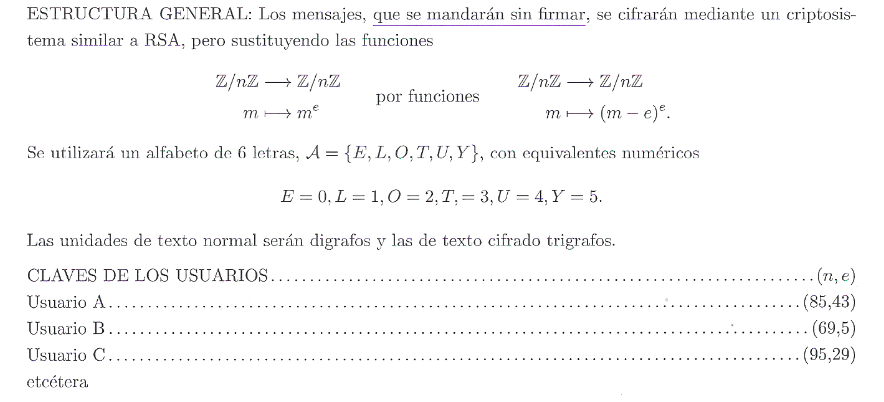
\includegraphics[width=\textwidth]{img/info_estructura_red_parcial.png}
\end{center}

Interceptamos un mensaje que el usuario $A$ ha enviado al usuario $B$, y que sabemos que termina con el nombre de $A$. El final del mensaje cifrado es $EOE$. ¿Cómo se llama el usuario $A$?
\solution

\doneby{Pedro}

% (85,43) -- (69,5)
Lo que tenemos que hacer es descifrar el mensaje $EOE$ para lo que necesitamos factorizar $n_B$.

Puesto que estamos trabajando con números pequeños es sencillo comprobar que $n_B=69 = 23\times 3$ con lo que tenemos $p=3$, $q = 23$.

A modo de comprobación, podemos ver que $e_B=5$ es coprimo con $(p-1)\cdot (q-1) = 44$.

Ahora calculamos el inverso de $e_B$:
\[d_B= \frac{1}{5} \mod 44 = 9\]

Este caso difiere un poco del caso habitual del algoritmo RSA visto en clase. Dado un mensaje $m$, el usuario $A$ envía a $B$ el valor
\[c = (m-e_B)^e_B\]
Para recuperar el valor de $m$, el usuario $B$ deberá calcular:
\[c^{d_B}+e_B = m-e_B+e_B = m\]

Una vez conocemos $e_B^{-1}$ podemos descifrar el mensaje:
\[EOE = 12 \mod 6^3 \]

\[f_{d_B}^{-1}(12) = (12)^9 + 5\mod 69 = 32 \mod 69 = 32 \mod 36 = YO\]

\end{problem}

\section{Hoja 4}
\begin{problem}[1]
 Una de las claves para que RSA funcione es el siguiente resultado:
 si $n=pq$, con $p,q$ primos distintos, y  $ed\equiv 1 \mod \phi(n)$, entonces $(m^e)^d\equiv m \mod n$ para cualquier entero $m$.

a) Sea ahora $N=mcm(p-1,q-1)$ [$mcm$=mínimo común múltiplo].
Demuestra que si  $ed'\equiv 1 \mod N$, entonces $(m^e)^{d'}\equiv
m \mod n$ para cualquier entero $m$.

b) Dados dos enteros cualesquiera $a,b$, describe un algoritmo
rápido para calcular $mcm(a,b)$, y explica por qué es rápido.
[SUGERENCIA: ¿Cuál es la relación entre $mcm(a,b), mcd(a,b)$ y
$ab$?] 
\solution


\end{problem}


\begin{problem}[2]
Encontrar la clave privada de un usuario  de un criptosistema basado en el RSA si su clave p\'ublica   es  $(7519, 35)$.

\solution

\doneby{Pedro}

Sabemos que, por definición del algoritmo RSA tenemos dos primos $p$, $q$ tales que:
\[\left\{ \begin{array}{l} 7519 = p \cdot q\\
35 = 1 \mod (p-1)(q-1)\end{array}\right.\]

Por la cuenta de la vieja podemos ver que $7519=73 \times 103$, por lo que ya conocemos $p$ y $q$. 

Ahora sólo tenemos que encontrar el inverso de 35 módulo $72 \cdot 102 = 7344$ para lo que podemos emplear el algoritmo de Euclides.

\[
\begin{array}{l}
7344 = 209\cdot 35 +29\\
35 = 1 \cdot 29 + 6 \\
29 = 4\cdot 6 + 5 \\
6 = 5 + 1 
\end{array} \implies \begin{array}{l}
1 = 6 - 5 \\
5 = 29 - 4 \cdot 6 \implies 1 = 5 \cdot 6-29\\
6 = 35 - 29 \implies 1 = 5\cdot 35 -6 \cdot 29 \\
29 = 7344 - 209 \cdot 35 \implies 1=1259 \cdot 35 -6\cdot 7344
\end{array}
\]

Así tenemos que la clave privada es $d=1259$

\end{problem}

\begin{problem}[3]
En la guía de una red de comunicaciones aparece la siguiente
información:

ESTRUCTURA GENERAL: Los mensajes se cifrarán mediante el
criptosistema RSA. Se utilizará el alfabeto castellano de 30
letras  con 0,\dots,14,\dots,26=A,\dots,Ñ,\dots,Z, 27=el punto,
28=espacio en blanco y 29=la interrogación. Las unidades de texto
normal serán digrafos y las de texto cifrado trigrafos. Los mensajes se mandan
{\bf sin firma}.

 CLAVES DE LOS
USUARIOS\dotfill$(n,e)$

Usuario A\dotfill(1711,125)

etcétera
\vspace{2mm}

  El usuario B envía el mensaje {\it ASÑAW.} al usuario A.   ¿Qué quiere decirle B a A?
\solution

\doneby{Pedro}

Lo que debemos hacer es encontrar los primos $p,q$ con los que se diseñó este sistema RSA.

Por la cuenta de la vieja llegamos a que $1711=p\cdot 1 = 29 \cdot 59$.

Una vez tenemos esto podemos conocer $(p-1)\cdot (q-1)=28 \cdot 58 = 1624$ lo que nos permite calcular la clave privada, que, en este caso, es el inverso de 125 módulo $1624$. Vamos a ello

\[
\begin{array}{l}
1624 = 12 \cdot 125 + 124\\
125 = 124 + 1
\end{array} \implies \begin{array}{l}
1 = 125 -124 \\
124 = 1624 - 12 \cdot 125 \implies 1 = 13 \cdot 125 - 1624
\end{array}
\]

Así tenemos que la clave privada, empleada para descifrar, será $d=13$. 

Para descifrar el mensaje procedemos por bloques:
\[19\cdot 30 + 14 = 584 \mod 1711 \to 584^13 \mod 1711 = 225 = 7\cdot 30 + 15 = HO\]
\[23 \cdot 30 + 27 = 717 \mod 1711 \to 717^13 \mod 1711 = 330 = 11 \cdot 30 + 0 = LA\]

Así tenemos que el mensaje enviado era ``HOLA''
\end{problem}

\begin{problem}[4]
En la guía de una red de comunicaciones aparece la
siguiente información:

ESTRUCTURA GENERAL: Los mensajes se cifrarán mediante el
criptosistema RSA. Se utilizará el alfabeto castellano de 26
letras (con Ñ y sin W). Las unidades de texto normal serán
digrafos y las de texto cifrado trigrafos. Los mensajes se mandan
{\bf firmados} (usando el protocolo explicado en clase).

 CLAVES DE LOS
USUARIOS\dotfill$(n,e)$\hphantom{(9797,17)(8549,6083)}

Usuario A\dotfill(9797,17)\hphantom{$(n,e)$(8549,6083)}

Usuario B\dotfill(8549,6083)\hphantom{(9797,17)$(n,e)$}

etcétera
\vspace{2mm}


  El usuario A envía un mensaje al usuario B y lo termina con
la firma EOBIXD. ?`Cómo se llama el usuario A?
\solution

\doneby{Pedro}

Para saber cómo se llama el usuario $A$ lo que tenemos que hacer es descifrar el mensaje para lo que debemos atacar al sistema RSA.

Procedemos a factorizar $n_B$ por la cuenta de la vieja obteniendo
\[n_B= 83 \cdot 103 = p \cdot q\]

A partir de aquí podemos calcular la clave privada calculando:
\[\frac{1}{e_b} \mod (p-1)(q-1) \equiv \frac{1}{6083} \mod 8364\]

Empleamos el algoritmo de Euclides para calcular este inverso:

\[
\begin{array}{l}
8364 = 1 \cdot 6083 + 2281 \\
6083 = 2\cdot 2281 + 1521 \\
2281 = 1\cdot 1521 + 760 \\
1521 = 2 \cdot 760 + 1
\end{array} \implies \begin{array}{l}
1 = 1521 -2\cdot 760 \\
760 = 2281 - 1521 \implies 1 = 3\cdot 1521 -2\cdot 2281 \\
1521 = 6083 - 2\cdot 2281 \implies 1 = 3 \cdot 6083 -8 \cdot 2281 \\
2281 = 8364 - 6083 \implies 1 = 11 \cdot 6083 - 8 \cdot 8364
\end{array}
\]

Por tanto tenemos que $d_B=11$. 

Puesto que el mensaje ha sido firmado lo que hemos recibido es 
\[\algb{C}=f_{d_A}(f_{e_B}(\algb{M}))\]

luego para descifrarlo debemos emplear primero la clave pública de $A$ y luego la privada de $B$, que acabamos de descubrir.

Una vez sabemos esto podemos descifrar el mensaje:
\[\begin{array}{l}
EOB = 3095 \mod n_A \to 3095^{17} \mod n_A = 1431 \mod n_A \to 1431^{11} \mod n_B = 255=``IP''\\
IXD = 6009 \mod n_A \to 6009^{17} \mod n_A = 1954 \mod n_A \to 1954^{11} \mod n_B = 12 = ``AN''
\end{array}\]


\end{problem}


\begin{problem}[5]
Un grupo de espias decide cifrar sus mensajes, escritos en
un alfabeto de 27 letras (las 26 del castellano, con Ñ y sin W, y
un espacio en blanco ``\_" que cifrarán como el 26), utilizando un
sistema de Vigenére sobre pares de letras. Para dificultar la
labor del enemigo, y en particular el análisis de frecuencias,
deciden cambiar la clave en cada mensaje. Para intercambiarse las
claves acuerdan utilizar el sistema RSA de clave pública. El
protocolo que utilizan es el siguiente:

Cuando $A$ quiere enviar a $B$ un mensaje $m$, busca una clave de
Vigenére, $K$, que será un par de letras $k_1k_2$. Esta clave le
da una función para cifrar $g_K$. Además $B$ tiene una función
pública para cifrar claves, $f_B$, cuya correspondiente función
para descifrar, $f^{-1}_B$, es secreta. $A$ interpreta $K$ (en
principio un par de letras) como un digrafo (un ``número de dos
cifras") al que puede aplicar $f_B$, y lo que envía a $B$ es el
par $(f_B(K),g_K(m))$. $B$ puede recuperar $K$ a partir de
$f_B(K)$, y una vez que conoce $K$ puede leer $m$ a partir de
$g_K(m)$.

\ppart Si las claves para cifrar son de la forma $(n,e)$, ?`Hay alguna
restricción sobre el tamaño de $n$?

\ppart Las primeras lineas de la guía de claves públicas para cifrar
claves de Vigenére dicen:

 Usuario
A\dotfill$((3^9-1)/2,3629)$\hphantom{$((2^{15}-1)/49,643)$$((3^9-1)/2,3629)$}


Usuario
B\dotfill$((2^{15}-1)/7,643)$\hphantom{$((3^9-1)/2,3629)$$((3^9-1)/2,3629)$}

 El usuario $B$ recibe el mensaje (AGR, TPXUROXK\_X). ?`Qué le han
querido decir?

\ppart Como acabas de comprobar, el protocolo anterior tiene un serio
problema de autentificación: cualquiera podría haber enviado el
mensaje. Discute si para resolver este problema es suficiente que
cuando $A$ escribe a $B$ envie el mensaje en la siguiente forma:
(Hola soy $A$, $f^{-1}_A(f_B(K)),g_K(m)$); o si hace falta
introducir alguna firma adicional. Discute también si siempre se
podrá utilizar $f^{-1}_A(f_B(K))$ o si habrá casos en los que
convenga sustituirlo por $f_B(f^{-1}_A(K))$. ?`Introduce esta
modificación alguna nueva restricción sobre el tamaño de las
posibles $n$ de las claves?

\ppart Supón que los espias han decidido cambiarse al nuevo protocolo
descrito en c), y que quien envió el mensaje de b) fue $A$. ?`Como
debería enviar ese mismo mensaje con el nuevo protocolo?
\solution

\end{problem}


\begin{problem}[6]
Supongamos que el alfabeto en claro tiene $29$ letras con
0,...,26=A,...,Z [alfabeto castellano], 27=espacio en blanco,
28=el punto, y que el alfabeto cifrado tiene $30$ letras,
añadiendo al anterior 29=?.   Las unidades de texto en claro serán
digrafos vistos como números de dos cifras en base $29$, es decir,
enteros entre $0$ y $840$ [o elementos de $\ent_{841}$].
Análogamente, las unidades de texto cifrado serán digrafos vistos
como enteros entre $0$ y $899$ [o elementos de $\ent_{900}$].
\begin{itemize}
\item[a)] El cifrado de $m$ es un entero $0\le f(m)\le  850$ tal que
$$f(m):=m^{13}+2 \pmod {851}.$$ (Notar que $(29)^2<851<(30)^2$.)
 Descifra el mensaje {\it LFNÑ}.
\item[b)]  ¿Es posible usar $g(m):=m^{11}+2 \pmod{851}$ para cifrar?
\end{itemize}
\solution

\doneby{Pedro}

\spart

Para poder descifrar la clave podemos suponer que estamos trabajando con un sistema $RSA$ (una vez le restemos 2 al mensaje cifrado estaremos ante un sistema RSA literalmente) con clave pública $e=13$ y $n=851$.

Procedemos a factorizar $851=p\cdot q = 37 \cdot 23$ por la cuenta de la vieja.

Ahora procedemos a calcular la clave privada:
\[d=\frac{1}{13} \mod 792 = 61\]

En esta ocasión es fácil ver que si multiplicamos por $13\cdot 60$ andamos cerca de $792$ y probando vemos rápido cuál es el inverso. 

Para quien no lo vea así de rápido siempre puede aplicar el algoritmo de Euclides.

Una vez conocemos la clave de descifrado procedemos a descifrar el mensaje:
\[\begin{array}{l} 
LF = 335 \mod 851 \to 335^61 \mod 851 = 37 = ``BI''\\
N\tilde{N} = 404 \mod 851 \to 404^{61} \mod 851 = 129 = ``EN''
\end{array}\]

\spart

Podemos ver que no es posible emplear la función $g$ para cifrar puesto que 
\[(p-1)(q-1) = 792 = 11\cdot 72\]

Por tanto, si tratásemos de emplear esta función para cifrar, al tratar de encontrar la clave privada veríamos que es imposible puesto que $e=11$ no es coprimo con $(p-1)(q-1)$.

 \end{problem}

\begin{problem}[7]
Supongamos que el alfabeto en claro tiene $29$
letras con 0,...,26=A,...,Z [alfabeto castellano], 27=espacio en
blanco, 28=el punto, y que el alfabeto cifrado tiene $30$ letras,
añadiendo al anterior 29=?   Las unidades de texto en claro serán
digrafos vistos como números de dos cifras en base $29$, es decir,
enteros entre $0$ y $840$ [o elementos de $\ent_{841}$].
Análogamente, las unidades de texto cifrado serán digrafos vistos
como enteros entre $0$ y $899$ [o elementos de $\ent_{900}$].
\begin{itemize}
\item[a)]  El cifrado de $m$ es un entero $0\le f(m)\le  852$ tal que
$$f(m):=m^{31}+2 \pmod {853}.$$ (Notar que $(29)^2<853<(30)^2$.)
 Descifra el mensaje {\it .CZE}
\item[b)]  ¿Es posible usar $g(m):=m^{32}+2 \pmod{853}$ para cifrar?
\end{itemize}
\solution
\end{problem}

%\begin{problem}
% Al cifrar los mensajes mediante el criptosistema RSA el primer número de las claves de los usarios $(n,e)$  es producto de 2 primos.

%1) ¿Porqué $n$ no puede ser un número primo?

%2) ¿Porqué no se usan claves con $n$ igual a producto de 3 primos?
%\end{problem}


\begin{problem}[8]
Probar que 15 es un pseudo-primo en base 4,
que 28 es un pseudo-primo en base 9 y que 91 es un pseudo-primo en
base 3.
\solution
\end{problem}

\begin{problem}[9]
Sea $n$ un número impar compuesto y sea $(b,n)=1$.

\ppart Sea $p$ un divisor primo de $n$ y escribamos $n'=n/p$. Probar que si $n$
es un pseudo-primo en base $b$ entonces $b^{n'-1}\equiv 1 \mod p$.

\ppart Demostrar que ningún entero de la forma $n=3p$, con $p>3$
primo, puede ser un pseudo-primo en bases 2, 5 ni 7.

\ppart Demostrar que ningún entero de la forma $n=5p$, con $p>5$
primo, puede ser un pseudo-primo en bases 2, 3 ni 7.

\ppart Probar que 91 es el menor pseudo-primo (impar) en base 3.

\solution
\end{problem}

\begin{problem}[10]
\ppart Probar que si $2^n-1$ es primo entonces $n$ es primo, y que si
$2^n+1$
 es primo entonces $n=2^k$. Los números $M_p:=2^p-1$, con $p$ primo, se
llaman ``números de Mersenne"\ y ``primos de Mersenne"\ en caso de
ser primos. Los de la forma $F_k:=2^{2^k}+1$ se llaman\ ``números
de Fermat"\ y\ ``primos de Fermat"\ si son primos. Los primeros
primos de Mersenne son 3,7, 31, 127, y todos los primos de Fermat
conocidos son 3, 5, 17, 257 y 65537.

\ppart Probar que todos los números de Fermat y todos los números de
Mersenne son pseudo-primos en base 2. (SUGERENCIA: Para los
números de Fermat, estudiar primero $2^{2^k} \mod F_k$, y
comprobar que podemos calcular $2^{F_k}$ a partir de este valor
por iteración de cuadrados. Para los de Mersenne, empezar por ver
que $p\vert M_p-1$ y deducir de ello que $M_p= 2^p-1\vert
2^{M_p-1}-1$.)

\ppart A pesar de lo anterior, comprobar que uno puede ver que $M_{11}=2047$ no es
primo utilizando un sencillo test de primalidad.

\solution

\end{problem}

%\begin{problem} 
%Sea $n$ un número de Carmichael. Demostrar que

%a) $n$ no es divisible por $m^2$ para ningun $m>1$;

%b) $n-1$ es divisible por $p-1$ para cualquier divisor primo $p$de $n$;

%c) $n$ es divisible por lo menos por 3 primos.
%\end{problem}

\begin{problem}[11]
\ppart Prueba que los siguientes son números de Carmichael: 561,
1729, 2465, 41041, 825265.



\ppart Demuestra que 561 es el menor número de Carmichael.

\solution
\end{problem}

\begin{problem}[12]
 Supongamos que $m$ es un entero positivo tal que $6m+1$, $12m+1$
y $18m+1$ son todos primos. Demostrar que $n=(6m+1)(12m+1)(18m+1)$
es un número de Carmichael. (Esta idea es una de las que han sido
utilizadas para intentar demostrar que hay infinitos números de
Carmichael, y durante mucho tiempo fue el método utilizado para
encontrar números de Carmichael muy grandes.)
\solution
\end{problem}

\begin{problem}[13]
Dado que es muy facil saber si un número par es primo o no (el
único par primo es el 2), no tiene demasiado sentido aplicar tests
de primalidad a los números pares. Sin embargo, y por aquello de
tener una teoría completa, se pide: demostrar que no existen
números de Carmichael pares, o sea, que para todo $n$ par existe
$b$ tal que $(b,n)=1$ y $b^{n-1}\not\equiv 1\mod n$.

\solution
\end{problem}

\begin{problem}[14]
Recordemos que la existencia de infinitos números de Carmichael es
un resultado reciente (Alford, Granville, Pomerance 1992). Sin
embargo, la existencia de infinitos pseudo-primos (verdaderos, o
sea, no primos) en base 2 era bien conocida. Posiblemente la
demostración más simple es la siguiente (Malo 1903): probar que si
$n$ es un pseudo-primo en base 2 compuesto, entonces $n':=2^n-1$
también es un pseudo-primo en base 2 compuesto. (SUGERENCIA: Tanto
la composición como la pseudo primalidad se basan en el hecho de
que si $a\vert b$ entonces $2^a-1\vert 2^b-1$, y en observar que
si $n$ es pseudo-primo en base 2 entonces $n\vert n'-1$.)
\solution
\end{problem}

\begin{problem}[15]
\ppart Encontrar los valores de $b$ para cuales $21$ es
pseudoprimo fuerte en base $b$.

\ppart  Encontrar los valores de $b$ para cuales $35$ es
pseudoprimo fuerte en base $b$.

\solution
\end{problem}

\begin{problem}[16]
Encontrar el menor primo mayor que 7674. (La idea es entender
cómo se buscan primos ``grandes", aunque he limitado el tamaño
para que podamos trabajar en la calculadora. Si tienes acceso a un
ordenador puedes buscar primos mayores (por ejemplo, de 6 cifras).
Las dos pistas son: buscar siempre los factores ``muy pequeños"\ y
recordar que el menor número que es pseudoprimo fuerte en bases 2
y 3 es $1.373.653=829\cdot1657$.)
\solution

\end{problem}

\vspace{2mm}

  Los dos ejercicios siguientes muestran que la
condición de pseudo-primalidad fuerte es mucho más restrictiva
que la de pseudo-primalidad, y cómo esto se puede aprovechar para
factorizar.

\vspace{2mm}

\begin{problem}[17]
Demuestra que 561, que es incluso un número de Carmichael, no es un
pseudo-primo fuerte en base 2. (De hecho, 561 solo es pseudo-primo
fuerte en 8 de las 318 bases no triviales posibles. Los otros dos
pseudo-primos en base 2 menores que 1000, o sea, 341 y 645,
tampoco son pseudo-primos fuertes en base 2.)
\solution
\end{problem}

\begin{problem}[18]
Prueba que si encontramos un $b$ tal que $n$ es pseudo-primo en base
$b$, pero no pseudo-primo fuerte en base $b$, entonces no es
difícil encontrar un factor no trivial de $n$.
\solution
\end{problem}
